\chapter{系统采样理论}
\thispagestyle{empty}

\section{采样过程与采样定理}
\subsection{采样过程}
如图\ref{信号采样},将连续信号转换成离散信号的过程,称为\dy[采样过程]{CYGC}。这个过程可以看成是一个信号的\dy[调制过程]{TZGC}。
\begin{figure}[!htb]
	\centering
	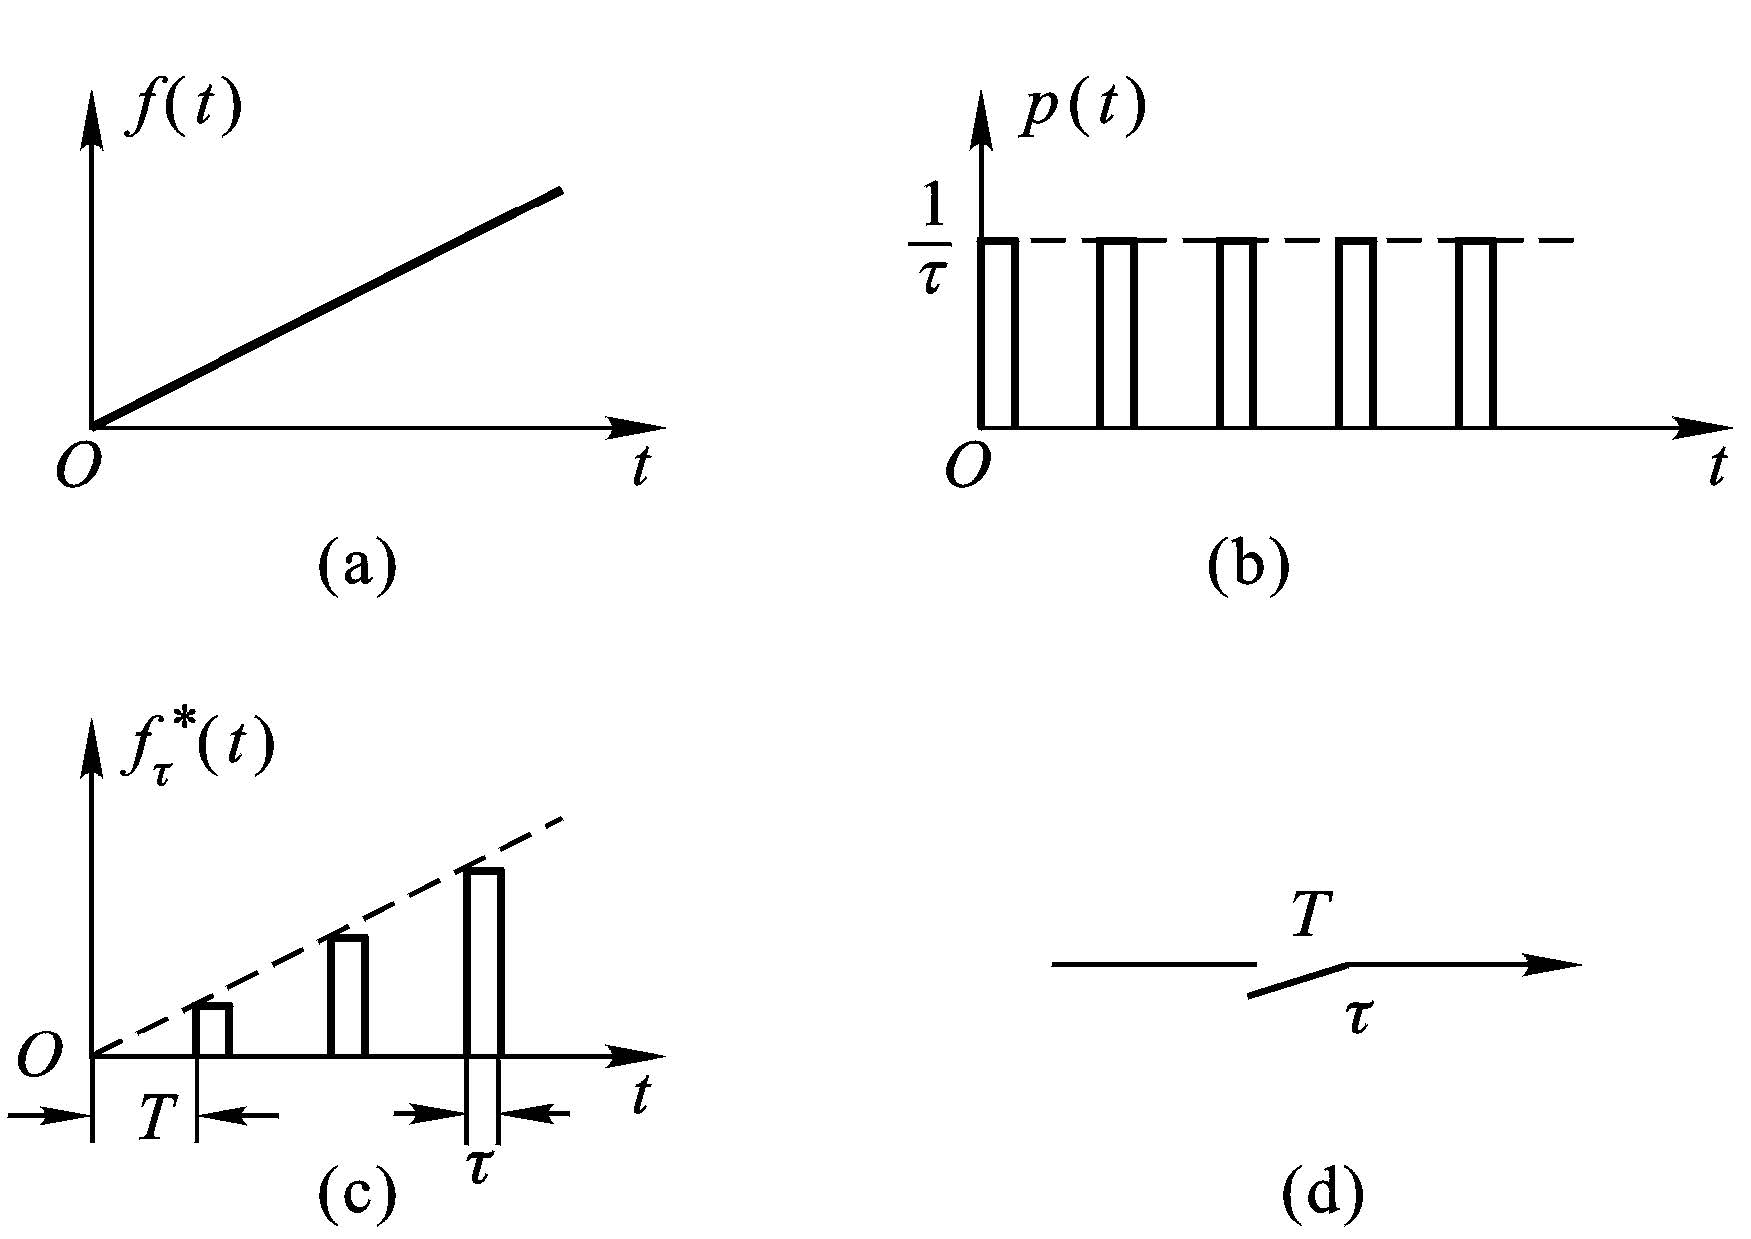
\includegraphics[width=0.6\linewidth]{pic/信号采样.jpg}
	\caption{信号的采样过程}
	\label{信号采样}
\end{figure}
\vspace*{-1em}
\begin{equation}
	f_\tau^*(t) = p(t) \cdot f(t)
\end{equation}
实现信号采样过程的装置称为\dy[采样开关]{CYKG},如图\ref{采样开关}.
\begin{figure}[!htb]
	\centering
	\begin{tikzpicture}
		\draw[arrows={-Stealth}] (0cm,0cm) --+(1cm,0cm)node[very near start, above = -4.5mm, xshift = -1.5mm]{$\tau$};
		\draw (-1.5cm, 0cm) -- (-0.5cm,0cm);
		\draw (-0.5cm, -0.2cm) -- (0cm,0cm)node[midway, above = 1mm]{$T$};
	\end{tikzpicture}
	\caption{采样开关}
	\label{采样开关}
\end{figure}

由于载波信号$p(t)$是周期函数,故可以展成如下Fourier级数
\begin{equation}
	p(t) = \sum_{n = -\infty}^{+\infty }C_n \e^{\j n \omega_\text{S} t}
\end{equation}
其中,$\omega_\text{S}= \dfrac{2\pi}{T}$,
\clearpage
\begin{align}
	C_n &= \dfrac{1}{T}\int_{T/2}^{-T/2}p(t)\e^{- \j n \omega_{\text{S}}t}\, \d t = \dfrac{1}{T}\int_{0}^{\tau} \e ^{- \j n \omega_{\text{S}}t}\, \d t \notag \\[0.5em]
	& = \dfrac{1}{T\tau}\cdot \dfrac{1}{- \j n \omega_{\text{S}}} \left(\e^{-\j n \omega_{\text{S}} \tau} - 1\right) = \dfrac{1}{T \tau} \cdot \dfrac{1}{-\j n \omega_{\text{S}}} \big(\cos n \omega_{\text{S}} \tau - \j \sin n \omega_{\text{S}} \tau - 1\big)\notag\\[0.5em]
	& = \dfrac{1}{T\tau}\cdot \dfrac{1}{-\j n \omega_{\text{S}}}\Bigg[1 - 2 \sin^2 \left(\dfrac{n \omega_{\text{S}} \tau}{2} \right)- 2 \j \sin \left(\dfrac{n \omega_{\text{S}} \tau}{2} \right) \cos \left(\dfrac{n\omega_{\text{S}}\tau}{2}\right) - 1\Bigg] \notag \\[0.5em]
	& = \dfrac{1}{T \tau} \cdot \dfrac{1}{-\j n \omega_{\text{S}}}(- 2 \j) \sin \left(\dfrac{n \omega_{\text{S}}\tau}{2}\right) \Bigg[\cos\left(\dfrac{n \omega_{\text{S}} \tau}{2}\right)- \j \sin \left(\dfrac{n \omega_{\text{S}} \tau}{2}\right)\Bigg]\notag\\[0.5em]
	& = \dfrac{1}{T} \dfrac{\sin\big(n\omega_{\text{S}}\tau /2\big)}{n \omega_{\text{S}} \tau / 2}\e^{-\j m \omega_\s \tau/2}
\end{align}

若连续信号$f(t)$的Fourier变换为$F(\j \omega)$,则采样信号$f_\tau^*(t)$的Fourier变换为
\begin{align}
	F_\tau^*(\j \omega) &= \int_{-\infty}^{+\infty} F_\tau^*(t)\e^{-\j \omega t}\, \d t = \int_{- \infty}^{+\infty} \Bigg[\sum_{n = -\infty}^{+ \infty}C_n f(t)\e^{\j n \omega_{\text{S}}t}\Bigg]\e^{-\j \omega t}\, \d t \notag \\[0.5em]
	& = \sum_{n = -\infty}^{+\infty} C_n \int_{-\infty}^{+\infty}f(t)\e^{-\j (\omega - n\omega_{\text{S}})t}\, \d t \notag \\[0.5em]
	& = \sum_{n = -\infty}^{+\infty} C_nF(\j \omega - \j n \omega_{\text{S}})
\end{align}

如图\ref{连续与离散信号},对于$n = 0$的部分,称为$F_\tau^*(\j \omega)$的\dy[主分量]{ZFL},其余的部分称为$F_\tau^*(\j \omega)$的\dy[补分量]{BFL}。
\vspace*{-1em}
\begin{figure}[!htb]
	\centering
	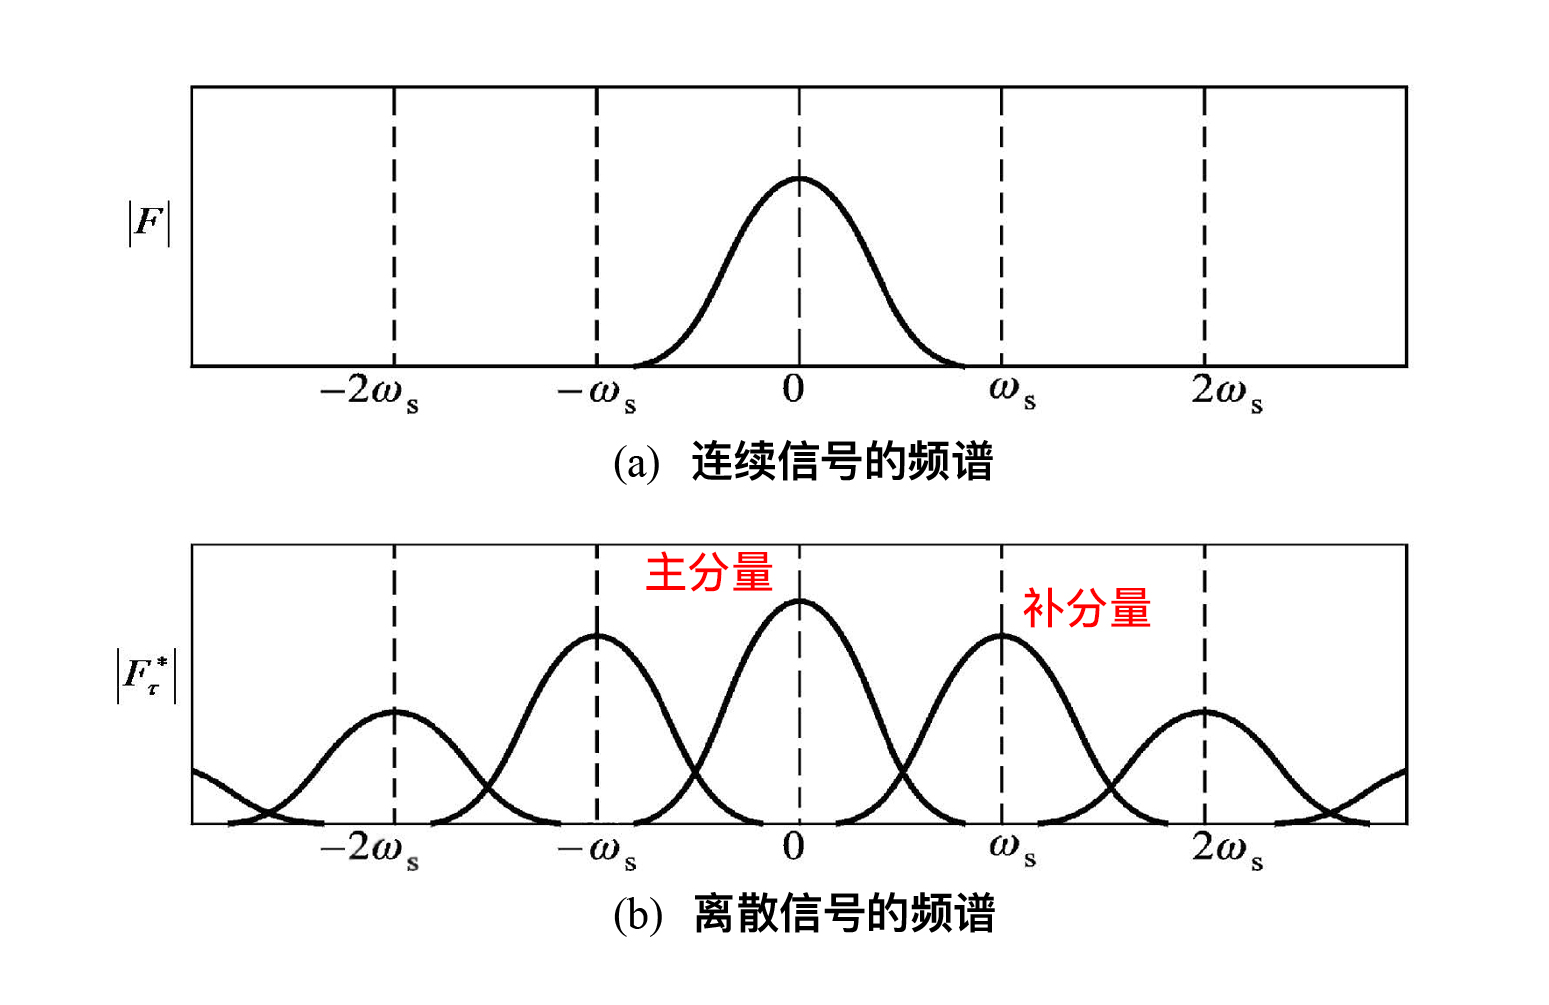
\includegraphics[width=0.7\linewidth]{pic/连续与离散信号.jpg}
	\vspace*{-2em}
	\caption{连续信号与离散信号的频谱($\omega_{\text{s}} < 2 \omega_\max$)}
	\label{连续与离散信号}
\end{figure}

\subsection{采样定理}
若存在一个理想的低通滤波器(其频率特性如图\ref{理想低通滤波器}),就可以将采样信号完全恢复成原连续信号。由此可得\dy[香农采样定理]{XNCYDL}:

如果采样频率$\omega_{\text{s}}$满足一下条件
\begin{equation}
	\omega_{\text{s}} \ge 2\omega_{\max}
\end{equation}
其中,$\omega_\max$为连续信号频谱的上限频率,此时离散信号和连续信号的频谱如图\ref{连续与离散信号2}.

则经采样得到的脉冲序列可以无失真地恢复为原连续信号。

\begin{figure}[!htb]
	\begin{minipage}{0.6\linewidth}
		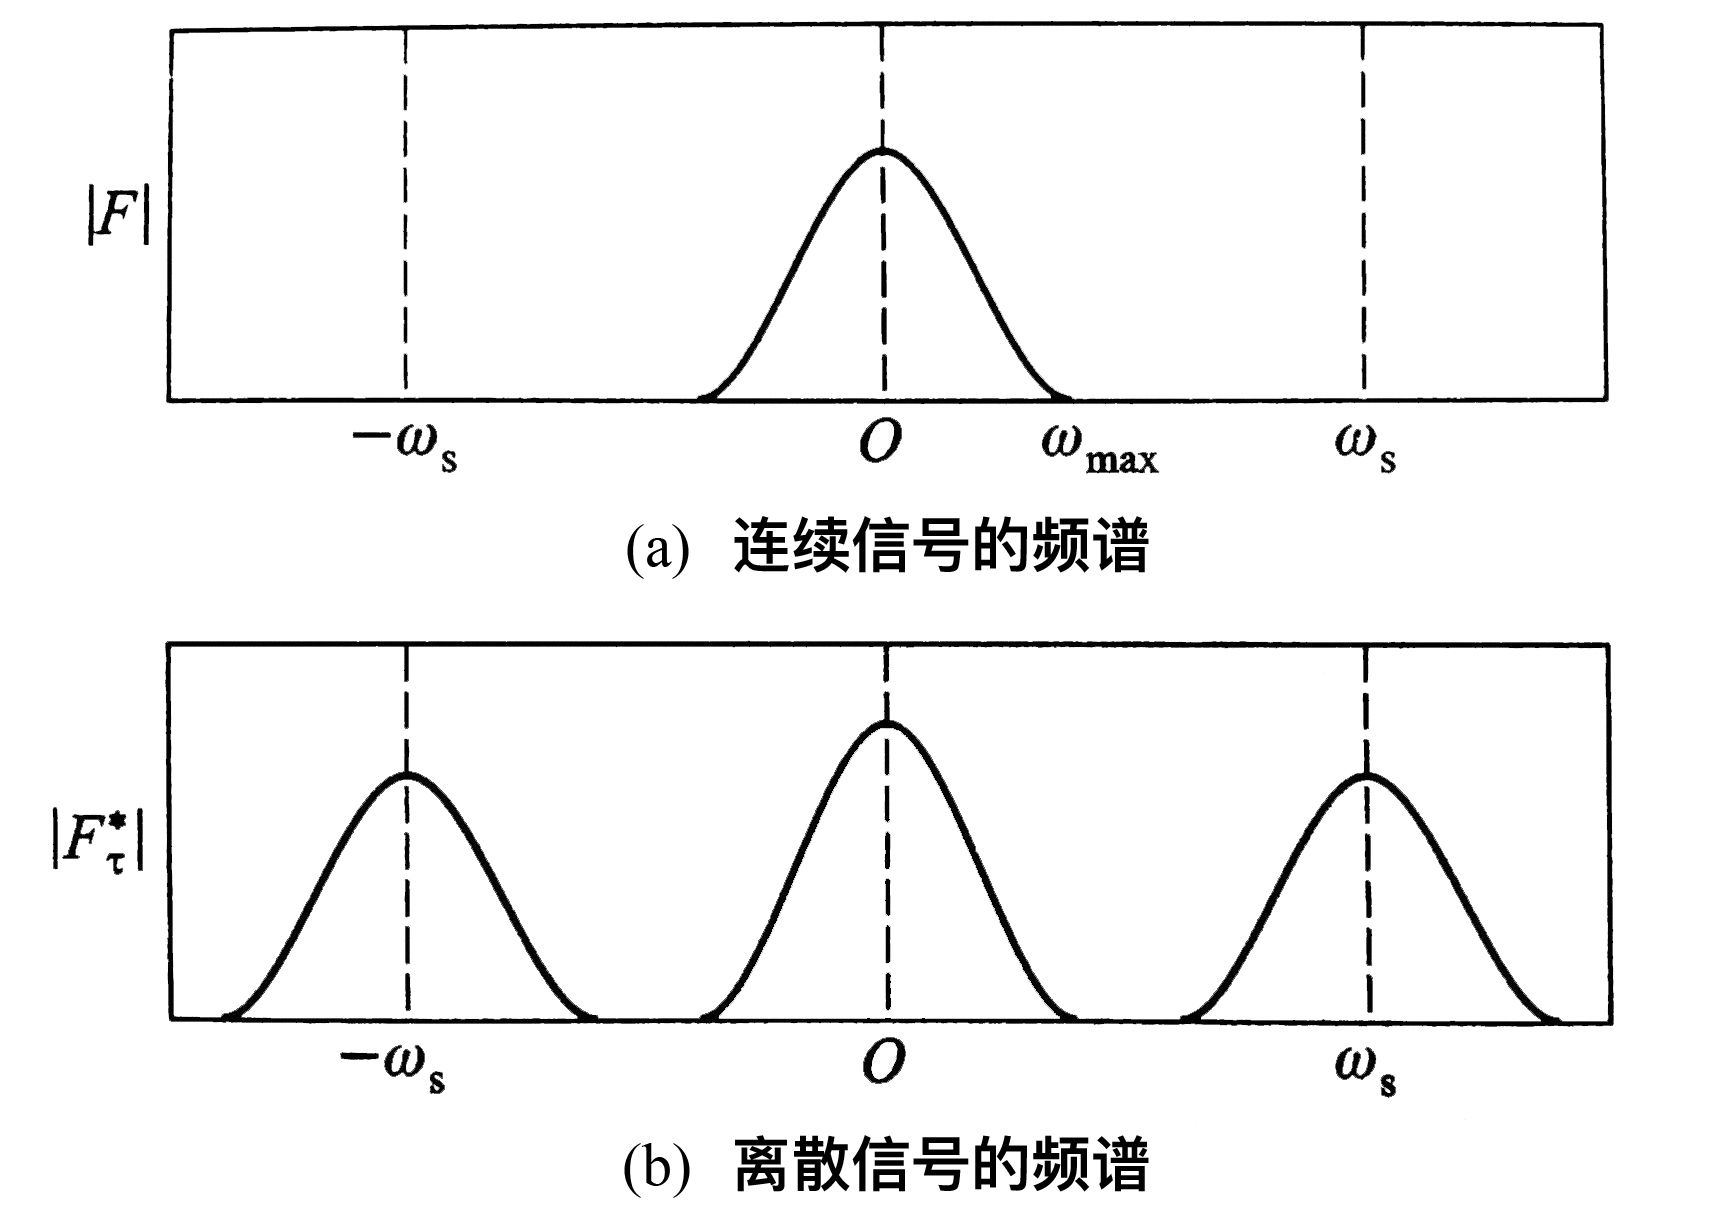
\includegraphics[width=\linewidth]{pic/连续与离散信号2.jpg}
		\vspace*{-1em}
		\caption{连续信号与离散信号的频谱($\omega_{\text{s}} \ge 2 \omega_\max$)}
		\label{连续与离散信号2}
	\end{minipage}
	\begin{minipage}{0.4\linewidth}
		\vspace*{11em}
		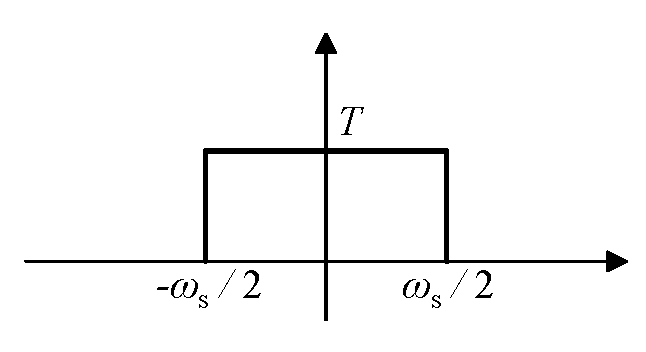
\includegraphics[width=\linewidth]{pic/理想低通滤波器.pdf}
		\vspace*{-1em}
		\caption{理想低通滤波器}
		\label{理想低通滤波器}
	\end{minipage}
\end{figure}
但理想的低通滤波器在物理上是不可实现的,在实际应用中只能用非理想的低通滤波器来代替理想的低通滤波器。

\subsection{理想采样过程}
为了简化采样过程的数学描述,引入\dy[理想采样开关]{LXCYKG}的概念。
\begin{figure}[!htb]
	\centering
	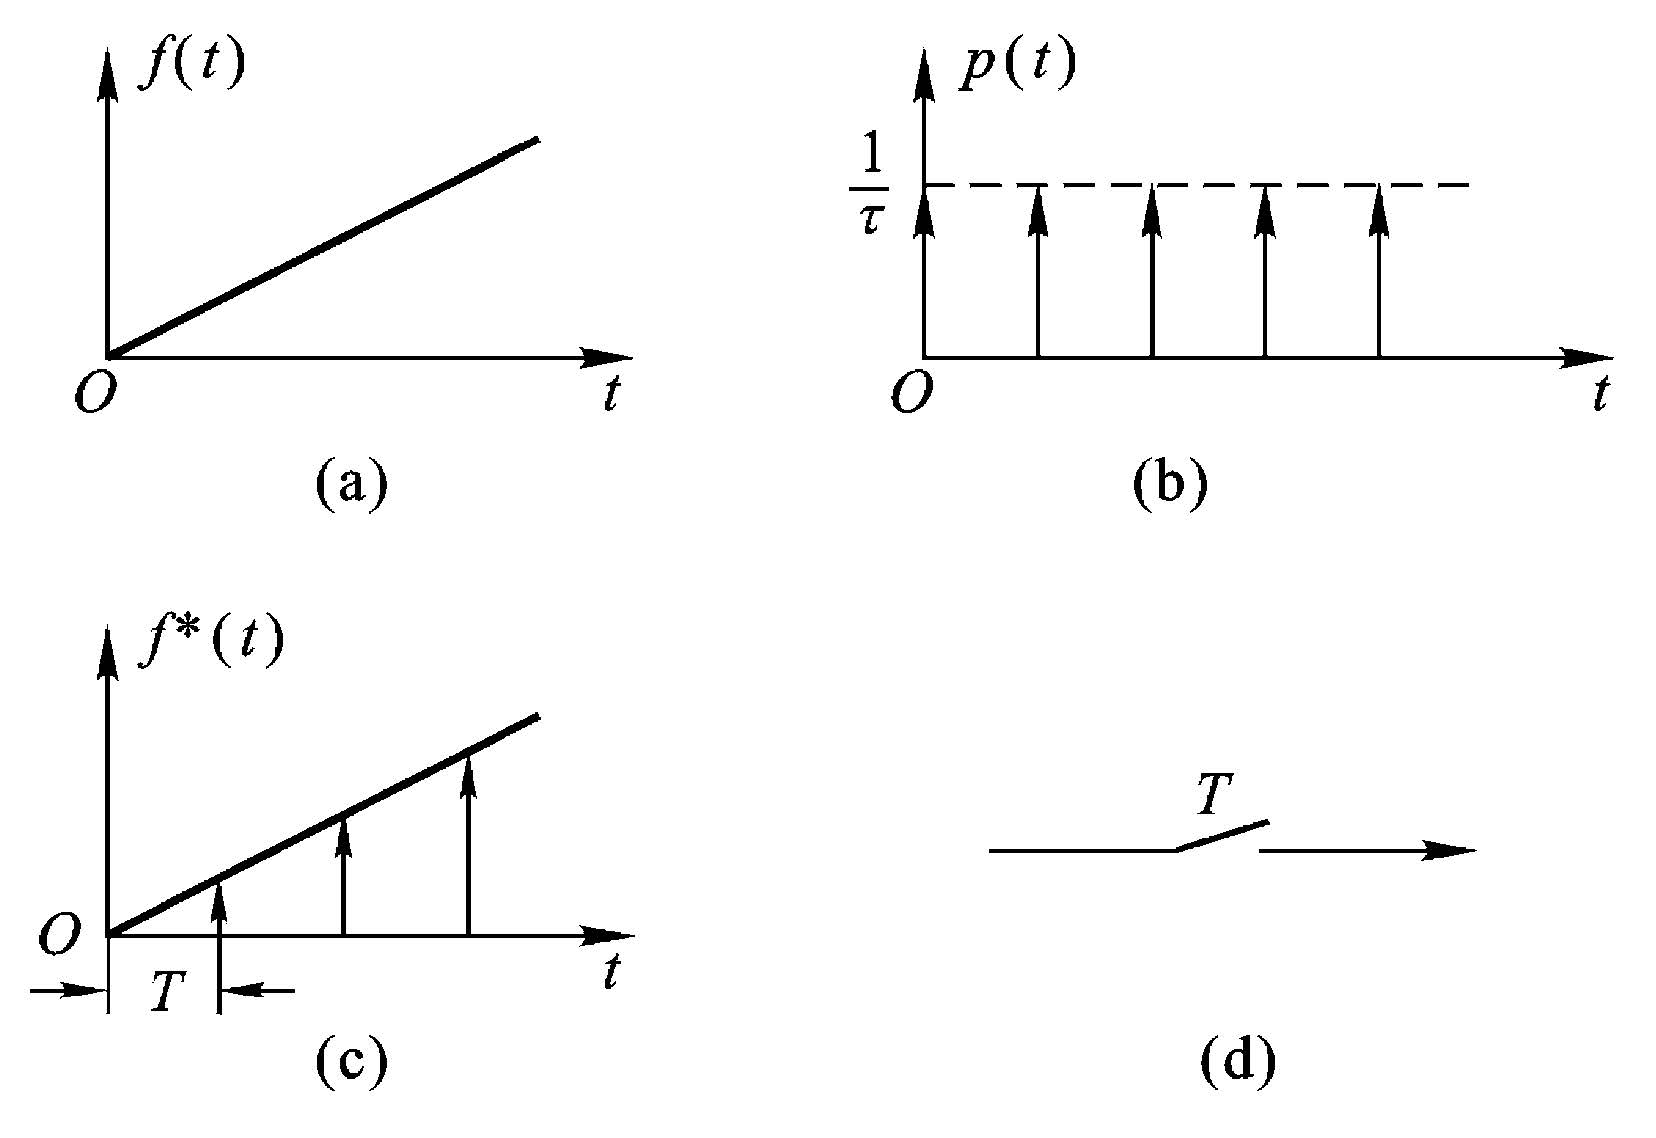
\includegraphics[width = 0.6\linewidth]{pic/理想采样开关.jpg}
	\vspace*{-0.5em}
	\caption{理想采样开关的采样过程}
	\label{理想采样开关的采样过程}
\end{figure}

\defination[理想采样开关]
载波信号$p(t)$可以近似成\dy[理想脉冲序列]{LXMCXL}
\begin{equation}
	\delta_T(t) = \sum_{k = -\infty}^{+\infty}\delta(t - kT)
\end{equation}
设当$t<0,f(t) = 0$,则
\begin{equation}
	f^*(t) = f(t) \cdot \delta_T(t) = \sum_{k = 0}^{\infty} f(t) \cdot \delta(t - kT)
\end{equation}
同样,$\delta_T(t)$可以展开成如下Fourier级数
\begin{equation}
	\delta_T (t) = \sum_{n = -\infty}^{+\infty}C_n \e^{\j n \omega_{\text{s}}t}
\end{equation}
其中,$C_n = \lim\limits_{\tau \to 0} \Bigg(\dfrac{1}{T}\dfrac{\sin(n\omega_\text{s}\tau /2)}{n \omega_\text{s}\tau/2}\e^{- \j n \omega_\text{s}\tau / 2}\Bigg) = \dfrac{1}{T}$.则有
\begin{align}
	f^*(t) = \dfrac{1}{T}\sum_{n = -\infty}^{+\infty}f(t)\e^{\j n \omega_\text{s}t}\\[0.5em]
	F^*(\j \omega) = \dfrac{1}{T}\sum_{n = -\infty}^{+\infty}F(\j \omega - \j n \omega_\text{s})
	\label{采样函数}
\end{align}

\section{信号的恢复与零阶保持器}
\subsection{信号恢复的基本概念}
\dy[信号恢复]{XHHF}是指采样信号恢复为连续信号的过程,能够实现这一过程的装置称为\dy[保持器]{BCQ}。对于$kT<t<(k+1)T$时,可将$f(t)$展开成泰勒级数
\begin{equation}
	f(t) = f(kT) + f'(t)\big|_{t = kT}\cdot(t - kT) + \cdots + \dfrac{1}{n!}f^{(n)}(t)\big|_{t = kT} \cdot (t-kT)^n + \cdots
\end{equation}
其中,各阶导数的近似值为
\begin{align}
	f'(kT) &\approx \dfrac{f(kT) - f(kT - T)}{T}\\[0.5em]
	f''(Kt) & \approx \dfrac{f'(kT) - f'(kT - T)}{T}\\
	& \quad \quad \cdots \cdots \notag
\end{align}
由此类推,计算$n$阶导数的近似值需已知$n+1$个采样时刻的瞬时值。

\subsection{零阶保持器}
\begin{figure}[!htb]
	\centering
	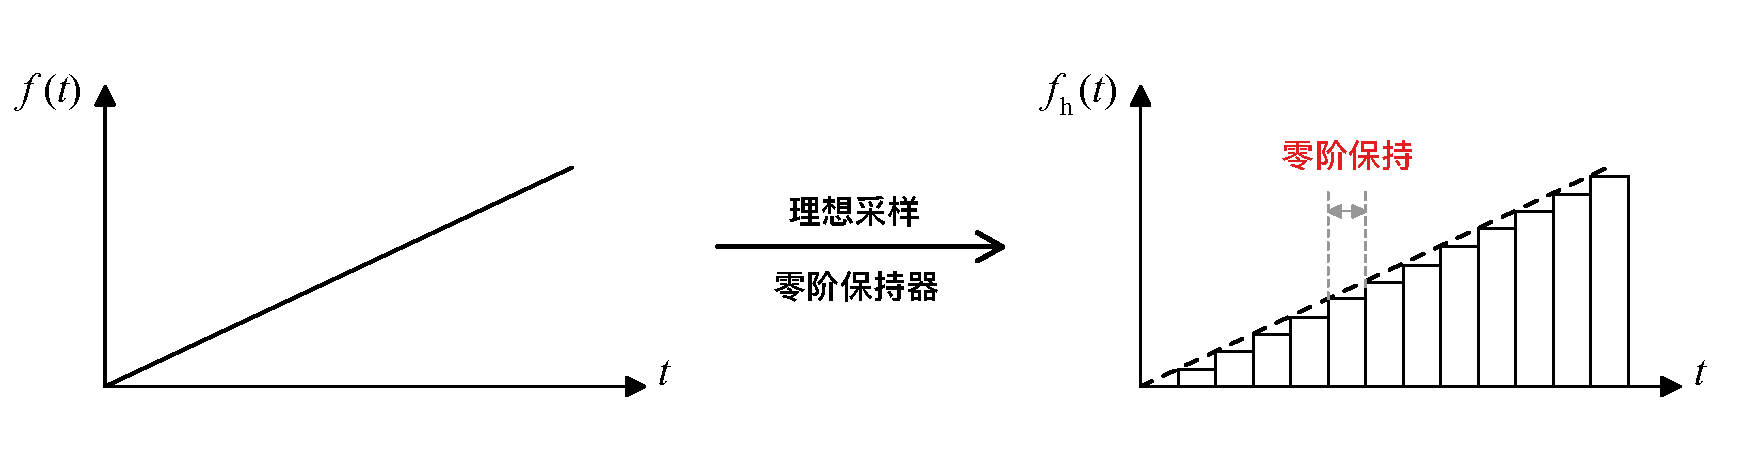
\includegraphics[width = 0.9\linewidth]{pic/零阶保持.pdf}
	\caption{零阶保持器采样示意图}
	\label{零阶保持器采样}
\end{figure}
零阶保持器的数学表达式为
\begin{equation}
	f(t) = f(kT), \quad kT < t<(k+1)T
\end{equation}
则理想采样开关的输出函数为
\begin{equation}
	f^*(t) = f(t)\cdot \delta_T(t) = \sum_{k = 0}^{\infty} f(kt) \cdot \delta(t - kT)
\end{equation}
其Laplace变换为
\begin{equation}
	F^*(s) = \sum_{k = 0}^{+\infty} f(kT) \e^{- kTs}
\end{equation}

\begin{figure}[!htb]
	\centering
	\begin{tikzpicture}
		\node (A)[draw, inner sep = 5pt, xshift = 2.5cm]{零阶保持器};
		
		\draw[arrows={-Stealth}] (0cm,0cm) --(A)node[midway, above = 0mm]{$f^*(t)$};
		\draw[arrows={-Stealth}] (A) -- +(2.2cm,0cm)node[midway, above = 0mm]{$f_\text{h} (t)$};
		\draw (-1.5cm, 0cm) -- (-0.5cm,0cm)node[very near start, above = 0cm]{$f(t)$};
		\draw (-0.5cm, -0.2cm) -- (0cm,0cm)node[midway, above = 1mm]{$T$};
		\draw[dashed] (-0.7cm, 0.5cm) -- (-0.7cm, -0.5cm) -- (0.2cm, -0.5cm)node[midway, above = -6mm]{\small 理想采样开关} -- (0.2cm,0.5cm) -- (-0.7cm, 0.5cm);
	\end{tikzpicture}
	\caption{零阶保持器}
	\label{零阶保持器}
\end{figure}
零阶保持器的输出为
\begin{equation}
	f_\text{h}(t) = \sum_{k = 0}^{+\infty} f(kT)\big[1(t- kT) - 1(t - kT - T)\big]
\end{equation}
其Laplace变换为
\begin{equation}
	F_\text{h}(s) = \sum_{k = 0}^{+ \infty}f(kT)\Bigg[\dfrac{\e^{-kTs} - \e^{-(k+1)Ts}}{s}\Bigg] = \Bigg(\dfrac{1 - \e^{- Ts}}{s}\Bigg) \sum_{k = 0}^{+\infty}f(kT)\e^{-kTs}
\end{equation}

则零阶保持器的传递函数为
\begin{equation}
	G_\text{h}(s) = \dfrac{F_{\text{h}}(s)}{F^*(s)} = \dfrac{1 - \e^{-Ts}}{s}
\end{equation}

\noindent 零阶保持器的频率特性为
\begin{align}
	G_\text{h} (\j \omega) = \dfrac{1 - \e^{\j \omega T}}{\j \omega} &= T \dfrac{\sin \big(\omega T / 2\big))}{\omega T /2} \e^{\textstyle -\frac{1}{2} \j \omega T} \notag \\[0.5em]
	&= T \dfrac{\sin \big(\pi \omega / \omega_\text{s}\big)}{\pi \omega / \omega_\text{s}}\e^{- \j \pi\omega /\omega_\text{s}}
\end{align}
\begin{itemize}
	\item 幅频特性
	\begin{equation}
		\big|G_\text{h}(\j \omega)\big| = T \Bigg|\dfrac{\sin \big(\pi \omega / \omega_\text{s}\big)}{\pi \omega / \omega_\text{s}}\Bigg|
	\end{equation}
	\item 相频特性
	\begin{equation}
		\angle G_\text{h}(\j \omega) = - \dfrac{\pi \omega}{\omega_\text{s}} + \angle \sin \big(\pi \omega / \omega_\text{s}\big)
	\end{equation}
	其中,
	\begin{equation}
		\angle \sin \big(\pi \omega / \omega_\text{s}\big) =
		\, \begin{cases}
			\,0, & 2n\omega_\text{s}<\omega < (2n+1)\omega_\text{s}\\[0.5em]
			\, \pi, & (2n+1)\omega_\text{s} < \omega < 2(n+1)\omega_\text{s}
		\end{cases}
		\quad (n = 0,1,2,\cdots)
	\end{equation}
\end{itemize}

零阶保持器的频率特性曲线如图\ref{零阶保持器幅频特性}所示,对比图\ref{理想低通滤波器}可知零阶保持器是一个低通滤波器,但不是理想的低通滤波器,它除了允许信号的主频谱分量通过外,还允许部分高频分量通过。
\begin{figure}[!htb]
	\centering
	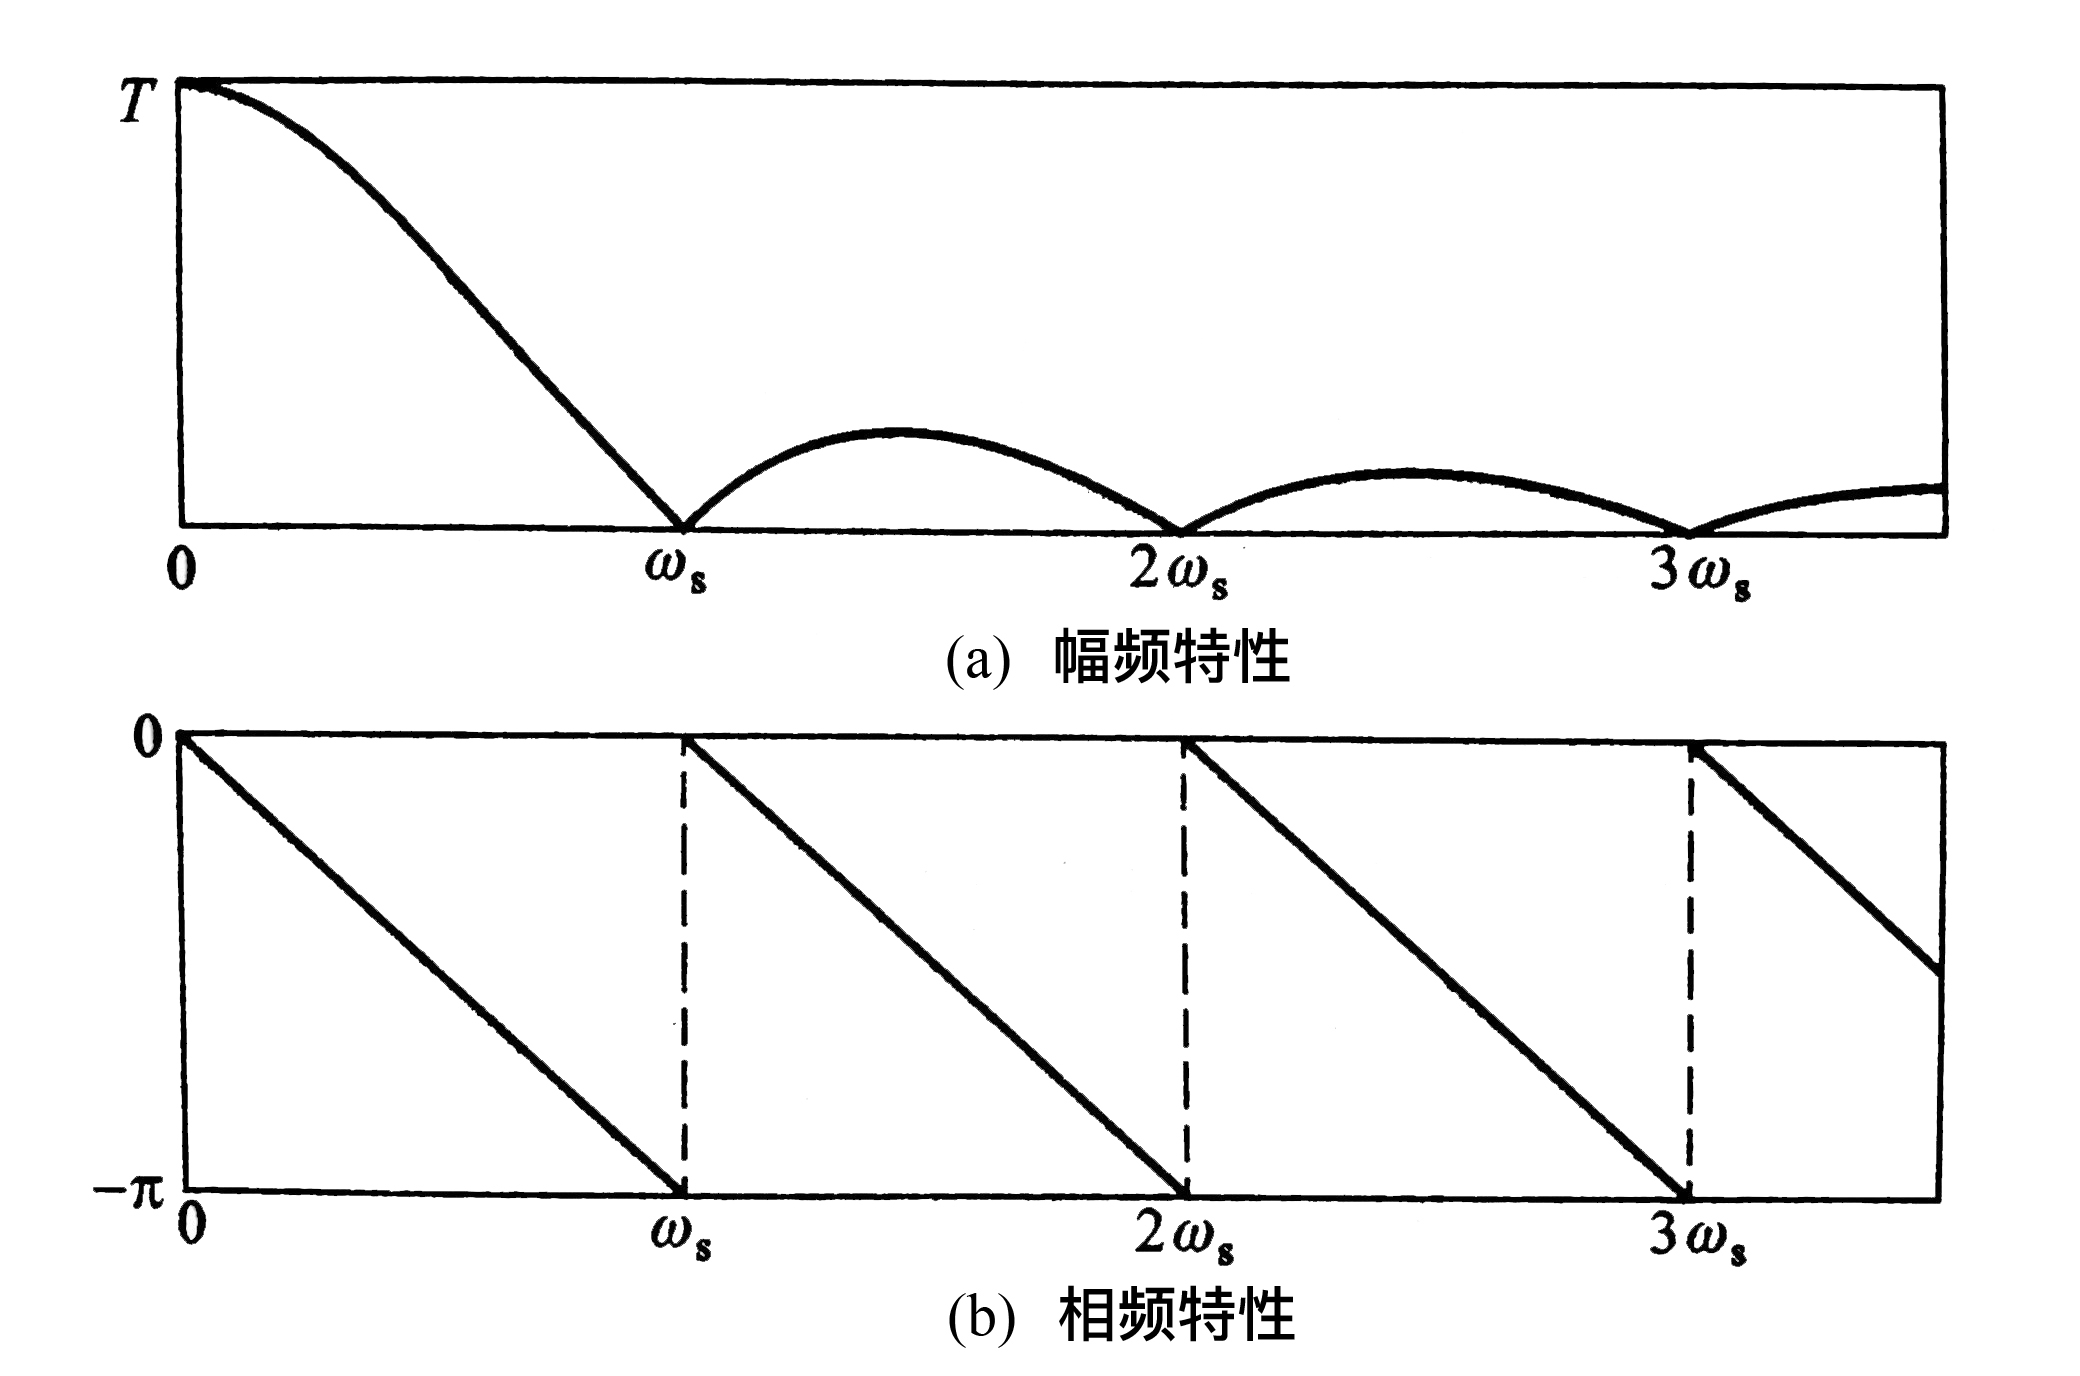
\includegraphics[width = 0.56\linewidth]{pic/零阶保持器幅频特性.jpg}
	\vspace*{-1em}
	\caption{零阶保持器的频率特性曲线}
	\label{零阶保持器幅频特性}
\end{figure}

\section{$z$变换与$z$逆变换}
\subsection{$z$变换}
连续信号$f(t)$经采样后得到的脉冲序列为
\begin{align}
	f^*(t) = \sum_{k = 0}^{+\infty}f(kT)\cdot \delta(t -kT)
\end{align}
对其进行Laplace变换,得
\begin{equation}
	F^*(s) = \sum_{k = 0}^{+\infty}f(kT)\e^{-kTs}
\end{equation}
引入一个新变量
\begin{equation}
	z = \e^{Ts}
\end{equation}
可得$z$变换的定义式
\begin{equation}
	F(z) = F^*(s)\big|_{s=(1/T)\ln z} = \sum_{k=0}^{\infty} f(kT)z^{-k}
\end{equation}
称$F(z)$为$f^*(s)$的\dy[$z$变换]{ZBH},记作$Z\big[f^*(t)\big]=Z\big[f(kT)\big]=F(z).$\\
求解方法:
\begin{enumerate}[\textbf{方法} 1 ]
	\item \textbf{级数求和法}\\
	展开以后是一个等比数列,求和以后再求极限即可求得$z$变换。
	\item \textbf{部分分式法}\\
	设连续函数的Laplace变换为有理函数,将其展开成\dy[部分分式]{BFFS}的形式为
	\begin{equation}
		F(s) = \sum_{i = 1}^{n} \dfrac{a_i}{s+s_i}
	\end{equation}
	因此,连续函数的$z$变换可以由有理函数求出
	\begin{equation}
		F(z) = \sum_{i=1}^{n} \dfrac{a_i z}{z - \e^{-s_iT}}
	\end{equation}
\end{enumerate}

\examples 求$f(t) = a^{t/T}$函数的$z$变换。

\solve 由$z$变换的定义有
\begin{align*}
	F(z) &= \sum_{k=0}^{\infty} f^*(kT)z^{-k} = \sum_{k = 0}^{\infty} a^{k} z^{-k}= \lim\limits_{k \to \infty} \dfrac{1 - (az^{-1})^{k+1}}{1-az^{-1}} = \dfrac{1}{1 - az^{-1}} = \dfrac{z}{z-a}
\end{align*}
\vspace*{1em}

\examples 求$F(s) = \dfrac{a}{s(s+a)}$的$z$变换。

\solve 将$F(s)$写成部分分式之和的形式
\[
F(s) = \dfrac{a}{s(s+a)} = \dfrac{1}{s} - \dfrac{1}{s+a}
\]
其中,$a_1 = 1,\quad a_2 = -1,\quad s_1 = 0, \quad s_2 = -a.$所以,
\[
F(z) = \dfrac{z}{z-1} - \dfrac{z}{z - \e^{-aT}} = \dfrac{(1 - \e^{-aT})z}{z^2 - (1 + \e^{-aT})z+\e^{-aT}}
\]

\subsection{常用信号的$z$变换}
常见函数的Laplace变换和Z变换如表\ref{常用函数的z变换}\footnote{请注意背诵此表,作者表示期末考栽在没有记住$Z\bigg[\dfrac{1}{s^3}\bigg]$上。}.

{
	\centering
	\setlength{\tabcolsep}{11mm}{
		\begin{longtable}{cccc}
			
			\toprule
			函数名 & $F(s)$ & $f(t)$ & $F(z)$\\
			\midrule
			\endfirsthead
			
			\multicolumn{3}{r}{续表}\\
			\toprule
			函数名 & $F(s)$ & $f(t)$ & $F(z)$\\
			\midrule
			\endhead
			
			% 表格“尾页前”,表格最后显示内容
			\bottomrule
			\endfoot
			
			% 表格“尾页”,表格最后显示内容
			\bottomrule
			\endlastfoot
			
			单位脉冲信号& 1& $\delta t$ & 1\\[1em]
			单位阶跃信号&$\dfrac{1}{s}$ & $1(t)$ & $\dfrac{z}{z - 1}\quad |z|>1$\\[1em]
			单位斜坡信号 & $\dfrac{1}{s^2}$ & $t$ & $\dfrac{Tz}{(z-1)^2} \quad |z|>1$\\[1em]
			单位加速度信号 & $\dfrac{1}{s^3}$ & $\dfrac{1}{2}t^2$ & $\dfrac{T^2z(z+1)}{2(z-1)^3} \quad |z|>1$\\[1em]
			指数函数 & $\dfrac{1}{s+a}$ & $\e^{-at}$ & $\dfrac{z}{z - \e^{-aT}}$\\[1em]
			正弦函数 & $\dfrac{\omega}{s^2 + \omega^2}$ & $\sin \omega t$ & $\dfrac{z \cdot \sin\omega T}{z^2 - 2z\cos \omega T + 1}$\vspace*{0,5em}
		\end{longtable}
	}
	\vspace*{-2em}
	\captionof{table}{常用函数的$z$变换}
	\label{常用函数的z变换}
}


\subsection{$z$变换的基本定理}
\begin{enumerate}[\hspace*{2em} \textbf{定理} 1 ]
	\item \textbf{线形定理}\\
	设$a_1,a_2$为任意常数,连续时间函数$f_1(t),f_2(t)$的$z$变换分别为$F_1(z),F_2(z)$,则有
	\begin{equation}
		Z\big[a_1f_1(t) + a_2f_2(t) \big] = a_1F_1(z)+a_2F_2(z)
	\end{equation}
	
	\item \textbf{滞后定理}\\
	设连续时间函数在$t < 0$时,$f(t) = 0$,且$Z\big[f(t)\big] = F(z)$,则有
	\begin{equation}
		Z\big[f(t-kT)\big] = z^{-k}F(z)
	\end{equation}
	
	\item \textbf{超前定理}\\
	设连续时间函数$f(t)$的$z$变换为$F(z)$,则有
	\begin{equation}
		Z\big[f(t+kT)\big] = z^kF(z) - \sum_{n = 0}^{k - 1} f(nT)z^{k-n}
	\end{equation}
	
	\item \textbf{初值定理}\\
	设连续时间函数$f(t)$的$z$变换为$F(z)$,则有
	\begin{equation}
		f(0) = \lim\limits_{z \to \infty} F(z)
	\end{equation}
	
	\item \textbf{终值定理}\\
	设连续时间函数$f(t)$的$z$变换为$F(z)$,则有
	\begin{equation}
		f(\infty) = \lim\limits_{z \to 1} (1 - z^{-1})F(z) = \lim\limits_{z \to 1}(z - 1)F(z)
	\end{equation}
	
	\item \textbf{位移定理}\\
	设$a$为任意常数,连续时间函数$f(t)$的$z$变换为$F(z)$,则有
	\begin{equation}
		Z\big[f(t)\e^{-at}\big] = F(z\cdot \e^{aT})
	\end{equation}
\end{enumerate}

\subsection{$z$逆变换}
$z$逆变换是$z$变换的逆运算。其目的是由像函数$F(z)$求出所对应的采样脉冲序列$f^*(t)$($f(kT)$),记作
\begin{equation}
	Z^{-1}\big[F(z)\big] = f^*(t)
\end{equation}
\vspace*{-2em}

\warn[\hspace*{2em}$z$逆变换只能求出采样信号$f^*(t)$,但不能求出连续信号$f(t)$。]

\noindent 求解方法:
\begin{enumerate}[\textbf{方法} 1 ]
	\item \textbf{部分分式法}\\
	若象函数$F(z)$是复变量$z$的有理分式,且$\dfrac{F(z)}{z}$的极点$z_i = \e^{-a_iT}$互异,则
	\begin{equation}
		\dfrac{F(z)}{z} = \dfrac{K_1}{z - \e^{-a_1T}} + \dfrac{K_2}{z - e^{-a_2T}} + \cdots + \dfrac{K_m}{z - \e^{-a_mT]}}
	\end{equation}
	其中,
	\begin{equation}
		K_i = \lim\limits_{z \to z_i} (z - z_i) \dfrac{F(z)}{z}
	\end{equation}
	两边同时乘以$z$,再取反变换得
	\begin{align}
		Z^{-1}\big[F(z)\big] &= Z^{-1}\Bigg[\dfrac{K_1z}{z-\e^{-a_1T}}\Bigg] + Z^{-1}\Bigg[\dfrac{K_2z}{z-\e^{-a_2T}}\Bigg] + \cdots + Z^{-1}\Bigg[\dfrac{K_mz}{z-\e^{-a_mT}}\Bigg]\\[1em]
		f(kT) &= K_1\e^{-a_1kT} + K_2 \e^{-a_2nT} + \cdots + K_m\e^{-a_mkT}
	\end{align}
	
	\item \textbf{长除法}\\
	若$z$变换函数$F(z)$是复变量$z$的有理函数,则可将$F(z)$展成$z^{-1}$的无穷级数,即
	\begin{equation}
		F(z) = f_0 + f_1z^{-1} + \cdots + f_k z^{-k} + \cdots
	\end{equation}
	则
	\begin{align}
		f(kT) &= f_k, \quad k = 0,1,2,\cdots\\
		f^*(t) &= \sum_{k = 0}^{+ \infty}f_k \delta(t - kT)
	\end{align}
	
	\item \textbf{留数计算法}\\
	由$z$变换的定义可知
	\begin{align}
		F(z) &= \sum_{k=0}^{+\infty} f(kT)z^{-k}\\
		F(z)z^{n-1} &= \sum_{k=0}^{+\infty}f(kT)z^{n-k-1}\\
		\oint_\Gamma F(z)z^{m-1}\,\d z &=\oint_\Gamma \Bigg[\sum_{k=0}^{+\infty}f(kT)z^{n-k-1}\Bigg]\,\d z = \sum_{k=0}^{+\infty} f(kT)\oint_\Gamma z^{n-k-1}\,\d z
	\end{align}
	根据柯西定理$\displaystyle \oint_\Gamma z^{n-1}\, \d z = 
	\,
	\begin{cases}
		\, 2\pi \j, &n = 0\\
		\, 0, & n \neq 0
	\end{cases}
	$,化简得
	\begin{align}
		f(kT) = \dfrac{1}{2\pi\j} \oint_\Gamma F(z)z^{k-1} \, \d z
	\end{align}
	其中,$\Gamma$包围了$F(z)z^{k-1}$的所有极点。设$F(z)z^{k-1}$的极点为$z_i,i=1,2,\cdots,n$,则
	\begin{align}
		f(kT) = \sum_{i=0}^n \text{Res}\big[F(z)z^{k-1},z_i\big]
	\end{align}
\end{enumerate}

\examples 求$F(z)=\dfrac{z}{(z-1)(z-\e^{-T})}$的逆变换。

\solve 首先将$\dfrac{F(z)}{z}$展成部分分式
\[
\dfrac{F(z)}{z} = \dfrac{K_1}{z-1} + \dfrac{K_2}{z-\e^{-T}}
\]
其中
\begin{align*}
	K_1 = \lim\limits_{z \to 1} (z-1)\dfrac{F(z)}{z} = \dfrac{1}{1- \e^{-T}}\\[0.5em]
	K_2 = \lim\limits_{z \to \e^{-T}} = - \dfrac{1}{1 - \e^{-T}}
\end{align*}
从而得到
\begin{align}
	F(z) = \dfrac{1}{1 - \e^{-T}}\Bigg(\dfrac{z}{z-1} - \dfrac{z}{z-\e^{-T}}\Bigg)\\[0.5em]
	f(nT) = \dfrac{1}{1 - \e^{-T}}\big(1 - \e^{-nT}\big)\\[0.5em]
	f^*(t) = \dfrac{1}{1 - \e^{-T}}\sum_{k = 0}^{+\infty} \big(1 - \e^{-kT}\big)\delta (t - kT)
\end{align}

\examples 求$F(z)=\dfrac{z}{(z-2)(z-3)}$的逆变换。

\solve 由于
\[
F(z) = \dfrac{z}{(z-2)(z-3)} = \dfrac{z}{z^2 -5z + 6} 
\]
运用长除法得
\[\left( {{z^2} - 5z + 6} \right)\mathop{\left){\vphantom{1\begin{array}{l}
z\\
\underline {z - 5 + 6{z^{ - 1}}} \\
\quad {\mkern 1mu} {\mkern 1mu} {\mkern 1mu} 5 - 6{z^{ - 1}}\\
\quad {\mkern 1mu} {\mkern 1mu} {\mkern 1mu} \underline {5 - 25{z^{ - 1}} + 30{z^{ - 2}}} \\
\quad \quad {\mkern 1mu} {\mkern 1mu} {\mkern 1mu} {\mkern 1mu} {\mkern 1mu} {\mkern 1mu} 19{z^{ - 1}} - 30{z^{ - 2}}\\
\quad \quad {\mkern 1mu} {\mkern 1mu} {\mkern 1mu} {\mkern 1mu} {\mkern 1mu} {\mkern 1mu} \underline {19{z^{ - 1}} - 95{z^{ - 2}} + 114{z^{ - 3}}} \\
\quad \quad \quad \quad \quad {\mkern 1mu} {\mkern 1mu} {\mkern 1mu} {\mkern 1mu} {\mkern 1mu} 65{z^{ - 2}} - 114{z^{ - 3}}\\
\quad \quad \quad \quad \quad {\mkern 1mu} {\mkern 1mu} {\mkern 1mu} {\mkern 1mu} {\mkern 1mu} \underline {65{z^{ - 2}} - 325{z^{ - 3}} + 390{z^{ - 4}}} \\
\quad \quad \quad \quad \quad {\mkern 1mu} {\mkern 1mu} {\mkern 1mu} {\mkern 1mu} \quad \quad {\mkern 1mu} {\mkern 1mu} {\mkern 1mu} {\mkern 1mu} {\mkern 1mu} {\mkern 1mu} {\mkern 1mu} {\mkern 1mu} {\mkern 1mu} {\mkern 1mu} {\mkern 1mu} {\mkern 1mu} 211{z^{ - 3}} - 390{z^{ - 4}}\\
\quad \quad \quad \quad \quad {\mkern 1mu} {\mkern 1mu} {\mkern 1mu} {\mkern 1mu} \quad \quad {\mkern 1mu} {\mkern 1mu} {\mkern 1mu} {\mkern 1mu} {\mkern 1mu} {\mkern 1mu} {\mkern 1mu} {\mkern 1mu} {\mkern 1mu} {\mkern 1mu} {\mkern 1mu} {\mkern 1mu} \quad \quad  \cdots  \cdots 
\end{array}}}\right.
\!\!\!\!\overline{\,\,\,\vphantom 1{\begin{array}{l}
z\\
\underline {z - 5 + 6{z^{ - 1}}} \\
\quad {\mkern 1mu} {\mkern 1mu} {\mkern 1mu} 5 - 6{z^{ - 1}}\\
\quad {\mkern 1mu} {\mkern 1mu} {\mkern 1mu} \underline {5 - 25{z^{ - 1}} + 30{z^{ - 2}}} \\
\quad \quad {\mkern 1mu} {\mkern 1mu} {\mkern 1mu} {\mkern 1mu} {\mkern 1mu} {\mkern 1mu} 19{z^{ - 1}} - 30{z^{ - 2}}\\
\quad \quad {\mkern 1mu} {\mkern 1mu} {\mkern 1mu} {\mkern 1mu} {\mkern 1mu} {\mkern 1mu} \underline {19{z^{ - 1}} - 95{z^{ - 2}} + 114{z^{ - 3}}} \\
\quad \quad \quad \quad \quad {\mkern 1mu} {\mkern 1mu} {\mkern 1mu} {\mkern 1mu} {\mkern 1mu} 65{z^{ - 2}} - 114{z^{ - 3}}\\
\quad \quad \quad \quad \quad {\mkern 1mu} {\mkern 1mu} {\mkern 1mu} {\mkern 1mu} {\mkern 1mu} \underline {65{z^{ - 2}} - 325{z^{ - 3}} + 390{z^{ - 4}}} \\
\quad \quad \quad \quad \quad {\mkern 1mu} {\mkern 1mu} {\mkern 1mu} {\mkern 1mu} \quad \quad {\mkern 1mu} {\mkern 1mu} {\mkern 1mu} {\mkern 1mu} {\mkern 1mu} {\mkern 1mu} {\mkern 1mu} {\mkern 1mu} {\mkern 1mu} {\mkern 1mu} {\mkern 1mu} {\mkern 1mu} 211{z^{ - 3}} - 390{z^{ - 4}}\\
\quad \quad \quad \quad \quad {\mkern 1mu} {\mkern 1mu} {\mkern 1mu} {\mkern 1mu} \quad \quad {\mkern 1mu} {\mkern 1mu} {\mkern 1mu} {\mkern 1mu} {\mkern 1mu} {\mkern 1mu} {\mkern 1mu} {\mkern 1mu} {\mkern 1mu} {\mkern 1mu} {\mkern 1mu} {\mkern 1mu} \quad \quad  \cdots  \cdots 
\end{array}}}}
\limits^{\displaystyle\hfill\,\,\, {{z^{ - 1}} + 5{z^{ - 2}} + 19{z^{ - 3}} + 65{z^{ - 4}} +  \cdots }}\]

则$f(0) = 0, \quad f(T) = 1, \quad f(2T) = 5, \quad f(3T) = 19, \quad f(4T) = 65, \cdots$,即
\[
f^*(t) = \delta(t-T) + 5\delta(t-2T) + 19\delta(t-3T) + 65\delta(t-4T) + \cdots
\]

\examples 求$F(z) = \dfrac{10z}{(z-1)(z-2)}$的逆变换。

\solve 采用留数计算法。
\[
F(z) z^{k-1} = \dfrac{10z^k}{(z-1)(z-2)}
\]
有两个极点$z_1 = 1,z_2 = 2$,且
\begin{align*}
	\text{Res}\big[F(z)z^{k-1}, 1\big] &= \lim\limits_{z \to 1}(z-1)F(z)z^{k-1} = -10\\
	\text{Res}\big[F(z)z^{k-1}, 2\big] &= \lim\limits_{z \to 2}(z-2)F(z)z^{k-1} = 10\cdot2^k
\end{align*}
所以
\[
f(kT) = 10(2^k - 1) \quad (k = 0,1,2,\cdots)
\]

\subsection{用$z$变换法解线性常系数差分方程}
\noindent \textbf{1. 差分的定义}

\defination[差分]
对误差信号$e(t)$进行采样,并将瞬时值$e(kT)$记为$e_k$或$e(k)$,则$e_k$的\\[0.5em]
一阶前向\dy[差分]{CF}定义为
\begin{equation}
	\Delta e_k = e_{k+1} - e_k
\end{equation}
二阶前向差分定义为
\begin{align}
	\Delta^2 \e_k &= \Delta\big(\Delta e_k\big) = \Delta e_{k+1} - \Delta e_k \notag\\
	&=e_{k+2} - 2e_{k+1}  + e_k
\end{align}
$n$阶前向差分定义为
\begin{equation}
	\Delta^n e_k = \Delta^{n-1}e_{k+1} - \Delta^{n-1}e_k
\end{equation}
一阶后向\dy[差分]{CF}定义为
\begin{equation}
	\nabla e_k = e_{k} - e_{k-1}
\end{equation}
$n$阶后向差分定义为
\begin{equation}
	\nabla^n e_k = \nabla^{n-1}e_{k} - \nabla^{n-1}e_{k-1}
\end{equation}

\noindent \textbf{2. 线性定常差分方程}

采样得到的到$k$时刻的所以输入数据记为$e_0,e_1,\cdots e_k$,对应的一直到$k-1$时刻的所有输出数据记为$u_0,u_1,\cdots u_{k-1}$,根据差分算法可以得到关于$u_k$的函数表达式
\begin{equation}
	u_k = f(e_0,e_1,\cdots, e_k,u_0,u_1,\cdots, u_{k-1})
\end{equation}
假设$u_k$是线性的,则其$n$阶\dy[线性差分方程]{XXCFFC}可表示为
\begin{equation}
	a_0u_k+a_1u_{k-1}+\cdots+a_nu_{k-n} = b_0e_k+b_1e_{k-1}+\cdots + b_me_{k-m}
\end{equation}

\noindent \textbf{3. 线性差分方程的求解}

\example[求解线性差分方程]\vspace*{0.5em}
\noindent  \hspace*{0.2em}  \tcbox[colframe =black, colback =black!10!white,boxrule=0.5mm,size=small,on line]{\color{black}{{ 解题步骤}}\hspace*{0.25em}}\hspace{1.5em}
\vspace*{0.5em}
\begin{enumerate}
	\item 对方程两边同时做$z$变换,注意利用$z$变换的超前定理
	\[
	Z\big[f(t+kT)\big] = z^kF(z) - \sum_{n = 0}^{k - 1} f(nT)z^{k-n}
	\]
	\item 求$C(z)$的$z$逆变换(三种方法,一般用留数计算法),得到$c(k)$。
\end{enumerate}

\examples 求解线性差分方程
\[
c(k+2) + 3c(k+1) + 2c(k) = 0
\]
初始条件为$c(0) = 0, c(1) = 1$.

\solve 对方程两边进行$z$变换,得
\[
z^2C(z) - z^2c(0)-zc(1)+3zC(z)-3zc(0)+2C(z) = 0
\]
代入初始条件$c(0) = 0, c(1) = 1$,化简后得
\[
C(z) = \dfrac{z}{z^2 + 3z + 2} = \dfrac{z}{(z+1)(z+2)} = \dfrac{z}{z+1} - \dfrac{z}{z+2}
\]
由留数计算法,求$C(z)z^{k-1}$的留数为
\begin{align*}
	\text{Res} \big[C(z)z^{k-1}, -1\big] &= \lim\limits_{z \to -1} (z+1)C(z)z^{k-1} = \lim\limits_{z \to -1} (z+1)\left(\dfrac{z}{z+1} - \dfrac{z}{z+2}\right)z^{k-1} = (-1)^k\\[0.5em]
	\text{Res} \big[C(z)z^{k-1}, -2\big] &= \lim\limits_{z \to -2} (z+2)C(z)z^{k-1} = \lim\limits_{z \to -2} (z+2)\left(\dfrac{z}{z+1} - \dfrac{z}{z+2}\right)z^{k-1} = 2(-2)^{k-1}=-(-2)^k
\end{align*}
所以最终解为
\[
c(k) = (-1)^k - (-2)^k\quad (k = 0,1,2,\cdots)
\]

\section{脉冲传递函数}
\subsection{脉冲传递函数的定义}

\begin{figure}[!htb]
	\centering
	\begin{tikzpicture}
		\node (A)[draw, inner sep = 5pt, xshift = 1.6cm]{$G(s)$};
		
		\draw[arrows={-Stealth}] (0cm,0cm) --(A)node[midway, above = 0mm]{$r^*(t)$};
		\draw[arrows={-Stealth}] (A) -- +(3cm,0cm)node[very near end, xshift = 0.6cm]{$c(t)$};
		\draw (-1.5cm, 0cm) -- (-0.5cm,0cm)node[midway, above = 0cm]{$r(t)$};
		\draw (-0.5cm, -0.2cm) -- (0cm,0cm);
		\draw[dashed] (2.5cm, 0cm) -- (2.5cm, 0.7cm) -- (3cm, 0.7cm);
		\draw (3cm, 0.5cm) -- (3.5cm,0.7cm);
		\draw[arrows={-Stealth}, dashed] (3.5cm, 0.7cm) -- (4.6cm,0.7cm)node[very near end, xshift = 0.5cm]{$c^*(t)$};

	\end{tikzpicture}
	\caption{开环采样系统}
	\label{开环采样}
\end{figure}

\defination[脉冲传递函数]
如图\ref{开环采样},输出采样信号$c^*(t)$的$z$变换与输入采样信号的$z$变换之比称为\dy[脉冲传递函数]{MCCDHS}
\begin{equation}
	G(z) = \dfrac{C(z)}{R(z)}
\end{equation}

\subsection{开环脉冲传递函数}
\noindent \textbf{1. 开环脉冲传递函数的推导}

由第\pageref{采样函数}页的公式\eqref{采样函数}可得
\begin{align}
	r^*(t) = \dfrac{1}{T}\sum_{n = -\infty}^{+\infty}r(t)\e^{\j n \omega_\text{s}t}\\[0.5em]
	R^*(s) = \dfrac{1}{T}\sum_{n = -\infty}^{+\infty}R(s - \j n \omega_\text{s})
\end{align}
由周期函数的定义可知$R^*(s)$是周期为$\j \omega_\text{s}$的周期函数。如图\ref{开环采样},连续环节的输出函数为
\begin{equation}
	C(s) = G(s)R^*(s)
\end{equation}
而
\begin{align}
	c^*(s) &= \dfrac{1}{T}\sum_{n = -\infty}^{+\infty}C(s - \j n \omega_\text{s}) = \dfrac{1}{T}\sum_{n = -\infty}^{+\infty}G(s - \j n \omega_\text{s}) R^*(s - \j n \omega_\text{s}) \notag \\[0.5em]
	& = \Bigg[\dfrac{1}{T}\sum_{n = -\infty}^{+\infty}G(s - \j n \omega_\text{s})\Bigg] R^*(s) =G^*(s)\cdot R^*(s)
\end{align}
即
\begin{equation}
	C(z) = G(z)R(z)
\end{equation}

\noindent \textbf{2. 串联环节的脉冲传递函数}
\begin{enumerate}[\hspace*{2em} (1) ]
	\item \textbf{串联环节间无采样开关时的脉冲传递函数}
	\begin{figure}[!htb]
		\centering
		\begin{tikzpicture}
			\node (A)[draw, inner sep = 5pt, xshift = 1.6cm]{$G_1(s)$};
			\node (B) [draw, inner sep =5pt, right of = A, node distance = 2.4cm]{$G_2(s)$};
			
			\draw[arrows={-Stealth}] (0cm,0cm) --(A);
			\draw[arrows={-Stealth}] (A) -- (B);
			\draw[arrows={-Stealth}] (B) --+(3cm,0cm);
			\draw (-1.5cm, 0cm) -- (-0.5cm,0cm);
			\draw (-0.5cm, 0cm) -- (0cm,0.2cm);
			\draw[dashed] (5cm, 0cm) -- (5cm, 0.7cm) -- (5.5cm, 0.7cm);
			\draw (5.5cm, 0.7cm) -- (6cm, 0.9cm);
			\draw [arrows={-Stealth},dashed] (6cm,0.7cm) -- (6.6cm,0.7cm); 
			\draw (0.3cm,1cm) --+(0cm,0.6cm);
			\draw (6.3cm,1cm) --+(0cm,0.6cm);
			\draw [arrows={Stealth-Stealth}] (0.3cm, 1.3cm) -- (6.3cm, 1.3cm)node[midway, above = 0cm]{$G(z)$};
			
			
		\end{tikzpicture}
		\caption{串联环节间无采样开关时的开环采样系统}
		\label{串联无开关}
	\end{figure}

	相当于把$G_1G_2$看作一个整体做$z$变换,其脉冲传递函数为
	\begin{equation}
		G(z) = Z\big[G_1(s)G_2(s)\big]=G_1G_2(z)
	\end{equation}
	\item \textbf{串联环节间无采样开关时的脉冲传递函数}
	\begin{figure}[!htb]
		\centering
		\begin{tikzpicture}
			\node (A)[draw, inner sep = 5pt, xshift = 1.6cm]{$G_1(s)$};
			\node (B) [draw, inner sep =5pt, right of = A, node distance = 2.4cm]{$G_2(s)$};
			
			\draw[arrows={-Stealth}] (0cm,0cm) --(A);
			\draw (A) -- +(0.9cm,0cm) --+(1.4cm, 0.2cm);
			\draw[arrows={-Stealth}] (3.cm, 0cm) -- (B);
			\draw[arrows={-Stealth}] (B) --+(3cm,0cm);
			\draw (-1.5cm, 0cm) -- (-0.5cm,0cm);
			\draw (-0.5cm, 0cm) -- (0cm,0.2cm);
			\draw[dashed] (5cm, 0cm) -- (5cm, 0.7cm) -- (5.5cm, 0.7cm);
			\draw (5.5cm, 0.7cm) -- (6cm, 0.9cm);
			\draw [arrows={-Stealth},dashed] (6cm,0.7cm) -- (6.6cm,0.7cm); 
			\draw (0.3cm,1cm) --+(0cm,0.6cm);
			\draw (6.3cm,1cm) --+(0cm,0.6cm);
			\draw [arrows={Stealth-Stealth}] (0.3cm, 1.3cm) -- (6.3cm, 1.3cm)node[midway, above = 0cm]{$G(z)$};
			
			
		\end{tikzpicture}
		\caption{串联环节间有采样开关时的开环采样系统}
		\label{串联有开关}
	\end{figure}
	
	其脉冲传递函数为各个连续环节z变换的乘积,记为
	\begin{equation}
		G(z) = Z\big[G_1(s)\big]Z\big[G_2(s)\big]=G_1(z)G_2(z)
	\end{equation}

	\item \textbf{有零阶保持器时的脉冲传递函数}
	\begin{figure}[!htb]
		\centering
		\begin{tikzpicture}
			\node (A)[draw, inner sep = 5pt, xshift = 1.6cm]{ZOH};
			\node (B) [draw, inner sep =5pt, right of = A, node distance = 2.4cm]{$G_2(s)$};
			
			\draw[arrows={-Stealth}] (0cm,0cm) --(A);
			\draw[arrows={-Stealth}] (A) -- (B);
			\draw[arrows={-Stealth}] (B) --+(3cm,0cm);
			\draw (-1.5cm, 0cm) -- (-0.5cm,0cm);
			\draw (-0.5cm, 0cm) -- (0cm,0.2cm);
			\draw[dashed] (5cm, 0cm) -- (5cm, 0.7cm) -- (5.5cm, 0.7cm);
			\draw (5.5cm, 0.7cm) -- (6cm, 0.9cm);
			\draw [arrows={-Stealth},dashed] (6cm,0.7cm) -- (6.6cm,0.7cm); 
			\draw (0.3cm,1cm) --+(0cm,0.6cm);
			\draw (6.3cm,1cm) --+(0cm,0.6cm);
			\draw [arrows={Stealth-Stealth}] (0.3cm, 1.3cm) -- (6.3cm, 1.3cm)node[midway, above = 0cm]{$G(z)$};
			
			
		\end{tikzpicture}
		\caption{含零阶保持器的开环采样系统}
		\label{串联零阶保持器开关}
	\end{figure}
\end{enumerate}

其开环传递函数为
\begin{align}
	G(z) &= \Bigg[\dfrac{1-\e^{-Ts}}{s}\cdot G(s)\Bigg] = Z\Bigg[\dfrac{1}{s}G(s)\Bigg] - Z\Bigg[\dfrac{1}{s}G(s)\e^{-Ts}\Bigg]\notag \\[0.5em]
	& = (1 - z^{-1})\cdot Z\Bigg[\dfrac{1}{s}G(s)\Bigg]
\end{align}

\subsection{闭环脉冲传递函数}
\begin{figure}[!htb]
	\centering
	\begin{tikzpicture}[circuit ee IEC]
		\node[bulb] (O) [draw, inner sep = 5pt, label = -85:$-$]{};
		\node (A) [draw, inner sep =6pt, right of = O, node distance =3cm]{$G(s)$};
		\node (B) [draw, inner sep = 6pt, below of = A, node distance = 1.5cm]{$H(s)$};
		
		\draw[arrows = {-Stealth}] (-1cm,0cm) -- (O)node[near start, above = 0mm]{$r(t)$};
		\draw (O) -- (1cm, 0cm) node[midway, above = 0mm]{$e(t)$} -- (1.5cm, 0.2cm);
		\draw[arrows = {-Stealth}] (1.5cm,0cm) -- (A)node[midway, above = 0cm]{$e^*(t)$};
		\draw[arrows = {-Stealth}] (A) --+(3cm, 0cm) node[very near end, xshift = 0.6cm]{$c(t)$};;
		\draw[arrows = {-Stealth}] (4.3cm, 0cm) -- +(0cm, -1.5cm) -- (B);
		\draw[arrows = {-Stealth}] (B) -- (0cm, -1.5cm) -- (O);
		\draw[dashed] (4.3cm,0cm) -- (4.3cm, 0.7cm)  -- (4.8cm, 0.7cm);
		\draw (4.8cm, 0.7cm) -- (5.3cm, 0.9cm);
		\draw[arrows = {-Stealth}, dashed] (5.3cm, 0.7cm) -- (6cm, 0.7cm)node[very near end, xshift = 0.5cm]{$c^*(t)$};;
		
	\end{tikzpicture}
\end{figure}

采样开关的输入和系统的输出分别为
\begin{align}
	E(s) &= R(s) - G(s)H(s)E^*(s)\\
	C(s) &= G(s) E^*(s)
\end{align}
可以得到
\begin{align*}
	E^*(s) &= R^*(s) - GH^*(s)E^*(s)\\
	C^*(s) &= G^*(s)E^*(s)
\end{align*}
整理得
\begin{equation}
	C^*(s) = \dfrac{G^*(s)}{1+GH^*(s)}R^*(s)
\end{equation}
即
\begin{align}
	C(z) &= \dfrac{G(z)}{1+GH(z)}R(z)\\[0.5em]
	\varPhi(z) &= \dfrac{C(z)}{R(z)} = \dfrac{G(z)}{1+GH(z)}
\end{align}

\example[求脉冲传递函数]
\examples \label{7.7}已知系统的结构图如图\ref{7.7.1},求输出脉冲函数$C(z)$.
\begin{figure}[!htb]
	\centering
	\begin{tikzpicture}[circuit ee IEC]
		\node[bulb] (O) [draw, inner sep = 5pt, label = -85:$-$]{};
		\node (A) [draw, right of = O, inner sep = 6pt, node distance = 2cm]{$G_1(s)$};
		\node (B) [draw, right of = A, inner sep = 6pt, node distance = 3cm]{$G_2(s)$};
		\node (C) [draw, below of = B, inner sep = 6pt, node distance = 1.5cm, xshift = -1.5cm]{$H(s)$};
		
		\draw [arrows={-Stealth}] (-1.5cm,0cm) -- (O)node[above = 0cm, near start]{$R(s)$};
		\draw [arrows={-Stealth}] (O) -- (A);
		\draw (A) -- (3.2cm,0cm) -- (3.7cm, 0.2cm);
		\draw [arrows={-Stealth}] (3.7cm, 0cm) -- (B);
		\draw [arrows={-Stealth}] (B) -- + (2cm,0cm)node[above = 0cm, very near end]{$C(s)$};
		\draw [arrows={-Stealth}] (6.3cm,0cm) -- +(0cm,-1.5cm) -- (C);
		\draw [arrows={-Stealth}] (C) -- (0cm,-1.5cm) -- (O);
		
	\end{tikzpicture}
	\caption{\ref{7.7}$\,\,$题系统结构图}
	\label{7.7.1}
\end{figure}

\solve 设采样前的信号为$E(s)$,采样后的信号为$E^*(s)$,则可以列出
\begin{align*}
	C(s) &= E^*(s) G_2(s)\\
	E(s) &= \big[R(s) - C(s)H(s)\big]G_1(s) = \big[R(s) - E^*(s)G_2(s)H(s)\big]G_1(s) = R(s)G_1(s) - E^*(s)G_2(s)H(s)G_1(s)
\end{align*}
对上面两个式子同时进行Z变换,可得
\begin{equation*}
	\begin{aligned}
		C(z) &= E(z)G_2(z)\\
		E(z) &= RG_1(z) - E(z)G_1G_2H(z)
	\end{aligned}
	\quad \Longrightarrow \quad
	E(z) = \frac{RG_1(z)}{1+G_1G_2H(z)}
	\quad \Longrightarrow \quad
	C(z) = \frac{G_2(z)RG_1(z)}{1+G_1G_2H(z)}
\end{equation*}


\section{采样系统的性能分析}
\subsection{稳定性}

\noindent \textbf{1. 从$s$平面到$z$平面的映射关系}

由$z$变换的定义
\begin{equation}
	z=\e^{Ts}
\end{equation}
令
\begin{equation}
	s = \sigma + \j \omega
\end{equation}
则
\begin{equation}
	z=\e^{\sigma T}\e^{\j \omega T}
\end{equation}
当$\sigma = 0$时,
\begin{equation}
	z = \e^{\j \omega T}
\end{equation}

此时$\omega: -\infty \to +\infty$,则$z$平面上的点绕单位圆逆时针绕无穷多圈。而当$\omega : -\dfrac{\omega_{\text{s}}}{2} \to \dfrac{\omega_\text{s}}{2}$时,则$z$平面上的点绕单位圆逆时针绕一圈。

由于闭环系统的特征根落在$s: \sigma < 0$的时候,系统稳定。即\textbf{如果闭环系统的特征根在$z$平面内的单位圆内,系统稳定。}其中,左半$s$平面上$ -\dfrac{\omega_{\text{s}}}{2} \le \omega \le \dfrac{\omega_\text{s}}{2}$的带称为\dy[主带]{ZD},其他部分称为\dy[次带]{CD}。
\vspace*{1.5em}

\noindent \textbf{2. $z$域的稳定条件和稳定性判据}

在$z$平面上系统稳定的充分必要条件是:系统的特征根必须全部位于$z$平面的单位圆内。

设采样系统的闭环脉冲传递函数为
\begin{equation}
	\varPhi(z) = \dfrac{C(z)}{R(z)} = \dfrac{M(z)}{D(z)}
\end{equation}
则闭环特征方程为$D(z) = 0.$
\begin{enumerate}[\hspace*{2em} (1) ]
	\item \dy[朱利稳定判据]{ZLWDPJ}\index{JURYWDPJ@Jury稳定判据}
	\begin{equation}
		D(z) = a_0 + a_1 z + a_2 z^2 + \cdots + a_n z^n
	\end{equation}
	且$a_n>0$,根据特征方程的系数构造朱利阵列,则方程$D(z) = 0$的根位于单位圆内的充分必要条件为
	\begin{equation}
		D_(1)>0, \quad (-1)^nD(-1)>0, \quad 
		\begin{cases}
			\, |a_0| < a_n\\
			\, |b_0| > |b_{n-1}|\\
			\, |c_0| > |c_{n-2}|\\
			\, \cdots\\
			\, |q_0| > |q_2|
		\end{cases}
	\end{equation} 
	
	\begin{table}
		\centering
		\setlength{\tabcolsep}{6.5mm}{
		\begin{tabular}{c|c|c|c|c|c|c|c}
			\hline
			行数 & $z^0$ & $z^1$ & $z^2$ & $\cdots$ & $\cdots$ & $z^{n-1}$ & $z^n$ \\
			\hline
			1& $a_0$ & $a_1$ & $a_2$ & $\cdots$ & $\cdots $ & $a_{n-1}$ & $a_n$\\
			2& $a_n$ & $a_{n-1}$ & $a_{n-2}$ & $\cdots$ & $\cdots $ &$a_1$ & $a_0$ \\
			3& $b_0$ & $b_1$ & $b_2$ & $\cdots$ & $\cdots $ & $b_{n-1}$ &  \\
			4& $b_{n-1}$ & $b_{n-2}$ & $\cdots$ & $\cdots $ &$b_1$ & $b_0$ & \\
			5& $c_0$ & $c_1$ & $c_2$ & $\cdots$ &  $c_{n-2}$ & &  \\
			6&$b_{n-2}$ & $\cdots$ & $\cdots $ &$b_1$ & $b_0$ & & \\
			$\cdots$ & $\cdots $& $\cdots$ &  $\cdots$ & $\cdots$ &  $\cdots$ & $\cdots$ &  $\cdots$ \\
			$2n-2$ & $q_2$ & $q_1$ & $q_0$ & & & & \\
			\hline
		\end{tabular}
		}
	\caption{朱利阵列}
	\label{朱利阵列}
	\end{table}
	其中,
	\begin{equation}
		b_k = 
		\begin{vmatrix}
			\,\, a_0 & a_{n-k} \,\,\\
			\,\, a_n & a_k \,\,
		\end{vmatrix}
		\quad \quad
		c_k = 
		\begin{vmatrix}
			\,\, b_0 & b_{n-1-k} \,\,\\
			\,\, b_{n-1} & b_k \,\,
		\end{vmatrix}
		\quad \quad \cdots
	\end{equation}

\item \dy[劳斯稳定判据]{RSWDPJ}\index{ROUTHWDPJ@Rough稳定判据}
\\
对于采样系统,也可用Routh判据分析其稳定性,但由于在z域中稳定区域是单位圆内,而不是左半平面,因此不能直接应用Routh判据。

引入双线性变换
\begin{equation}
	z = \dfrac{w + 1}{w - 1}
\end{equation}
此时可用Routh判据判断采样系统的稳定性。$s$平面、$z$平面、$w$平面的稳定区域如图\ref{三平面}所示。
\begin{figure}[!htb]
	\centering
	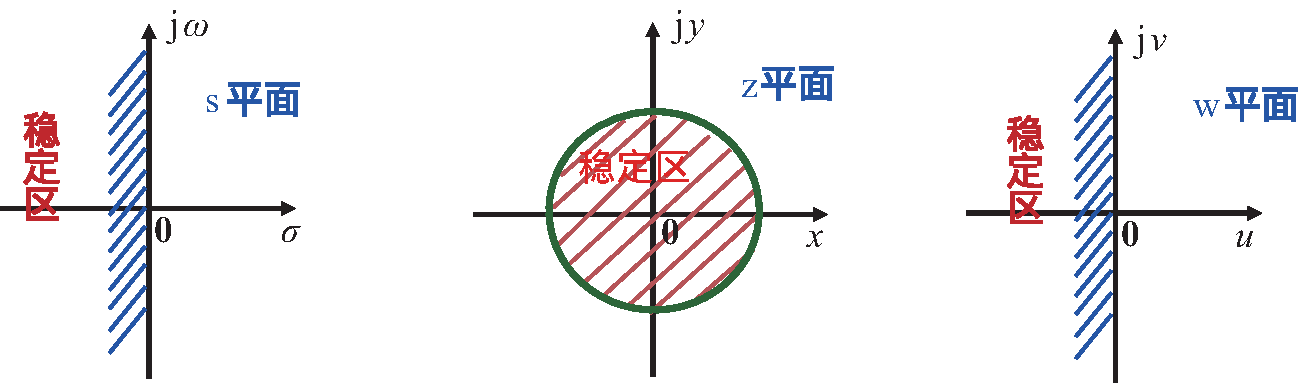
\includegraphics[width=0.7\linewidth]{pic/三平面.pdf}
	\caption{$s$平面、$z$平面、$w$平面的稳定区域}
	\label{三平面}
\end{figure}

\item $z$平面的根轨迹方法

根轨迹是当系统当特征方程当某些实参数由零变化到无穷时,特征根在复平面上移动的轨迹。
\begin{figure}[!htb]
	\centering
	\begin{tikzpicture}[circuit ee IEC]
		\node[bulb] (O) [draw, inner sep = 5pt, label = -85:$-$]{};
		\node (A) [draw, inner sep =6pt, right of = O, node distance =3cm]{$G(s)$};
		\node (B) [draw, inner sep = 6pt, below of = A, node distance = 1.5cm]{$H(s)$};
		
		\draw[arrows = {-Stealth}] (-1cm,0cm) -- (O)node[near start, above = 0mm]{$r(t)$};
		\draw (O) -- (1cm, 0cm) node[midway, above = 0mm]{$e(t)$} -- (1.5cm, 0.2cm);
		\draw[arrows = {-Stealth}] (1.5cm,0cm) -- (A)node[midway, above = 0cm]{$e^*(t)$};
		\draw[arrows = {-Stealth}] (A) --+(3cm, 0cm) node[very near end, xshift = 0.6cm]{$c(t)$};;
		\draw[arrows = {-Stealth}] (4.3cm, 0cm) -- +(0cm, -1.5cm) -- (B);
		\draw[arrows = {-Stealth}] (B) -- (0cm, -1.5cm) -- (O);
		\draw[dashed] (4.3cm,0cm) -- (4.3cm, 0.7cm)  -- (4.8cm, 0.7cm);
		\draw (4.8cm, 0.7cm) -- (5.3cm, 0.9cm);
		\draw[arrows = {-Stealth}, dashed] (5.3cm, 0.7cm) -- (6cm, 0.7cm)node[very near end, xshift = 0.5cm]{$c^*(t)$};;
		
	\end{tikzpicture}
	\caption{闭环采样系统}
	\label{闭环采样}
\end{figure}

如图\ref{闭环采样}所示,以基本的闭环采样系统为例,其特征方程为
\begin{equation}
	1+G(z) = 1+GH(z) = 0
\end{equation}
其与$s$平面所得到的根轨迹方程(见第\pageref{GH}页的公式\eqref{GH})形式完全一致。所以,\textbf{$z$平面和$s$平面中绘制根轨迹图的方法完全一致,只是在分析系统稳定性时,特征根位置的意义不同}。
\end{enumerate}

\examples \label{7.8}已知采样系统的闭环特征方程为
\[
D(z) = -0.125+0.75z-1.5z^2+z^3
\]
判断系统的稳定性。

\solve 由于$D(1) = 0.125 > 0, \quad (-1)^3D(-1) = 3.375>0$,求得朱利阵列如表\ref{7.8.1}.
\begin{table}[!htb]
	\centering
	\setlength{\tabcolsep}{6.5mm}{
		\begin{tabular}{c|c|c|c|c}
			\hline
			行数 & $z^0$ & $z^1$ & $z^2$ & $z^3$ \\
			\hline
			1& -0.125&0.75&-1.5&1\\
			2& 1&-1.5&0.75&-0.125\\
			3& -0.98&1.41&-0.56&\\
			4&-0.56 & 1.41 & -0.96&\\
			\hline
		\end{tabular}
	}
	\caption{\ref{7.8}$\,$的朱利阵列}
	\label{7.8.1}
\end{table}

由$|a_0| = 0.125<a_3=1,\quad |b_0| = 0.98 > |b_2| = 0.56$,所以系统是稳定的。
\vspace*{1em}

\examples 已知系统的闭环特征方程为
\[
D(z) = 45z^3 -117z^2+119z-39 = 0
\]
判断系统的稳定性。

\solve 将$z = \dfrac{w+1}{w-1}$代入特征方程式,得
\begin{align*}
	D(w) = 45 \left(\dfrac{w+1}{w-1}\right)^3 - 117 \left(\dfrac{w+1}{w-1}\right)^2 + 119\left(\dfrac{w+1}{w-1}\right) - 39 = 0\\
	45(w+1)^3-117(w+1)^2(w-1)+119(w+1)(w-1)^2-39(w-1)^3=0
\end{align*}
整理得
\[
w^3 + 2w^2 + 2w + 40 = 0
\]
列出劳斯表如下:
\begin{center}
	\begin{tabular}{ccc}
		$w^3$ & 1&2\\
		$w^2$ & 2&40\\
		$w^1$ & -18&\\
		$w^0$ & 40 &\\
	\end{tabular}
\end{center}
由劳斯判据可得:有2个根在$w$右半平面,即有2个根在$z$平面上的单位圆外,故系统为不稳定。
\vspace*{1em}

\examples \label{7.10}若已经求得系统的$G(z) = GH(z) = \dfrac{0.632Kz}{(z-1)(z-0.368)}$,绘制系统的根轨迹。

\solve 由根轨迹绘制的基本法则(见第\pageref{根轨迹的基本法则}页的章节\ref{根轨迹的基本法则}\nameref{根轨迹的基本法则}),可以绘制根轨迹如图\ref{7.10-1}。
\begin{figure}[!htb]
	\centering
	\vspace*{-1em}
	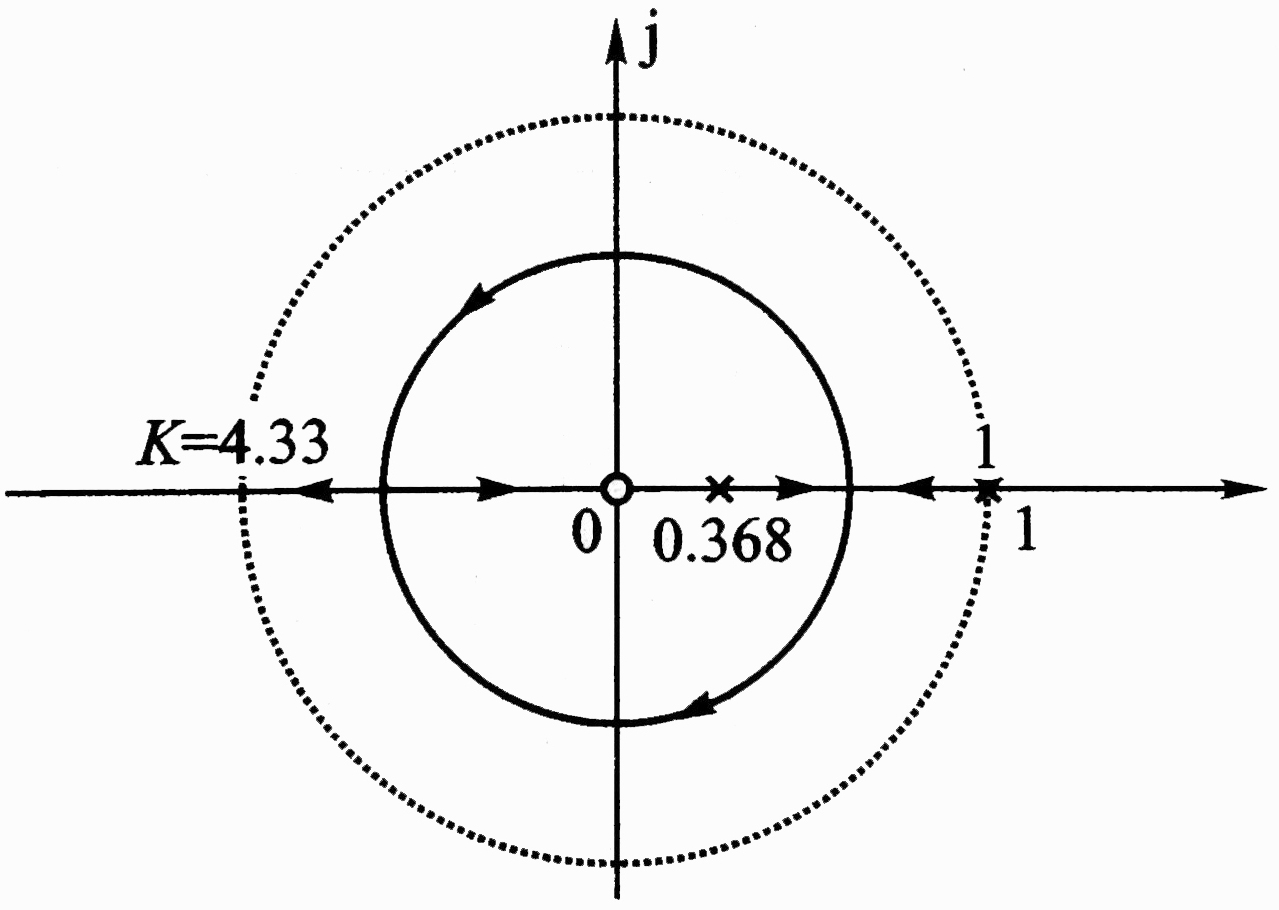
\includegraphics[width=0.3\linewidth]{pic/7-10根轨迹.jpeg}
	\vspace*{-1em}
	\caption{\ref{7.10}$\,$ 系统的根轨迹}
	\label{7.10-1}
\end{figure}

\subsection{闭环极点与瞬态响应之间的关系}
设采样系统的闭环传递函数为
\begin{align}
	\varPhi(z) &= \dfrac{b_0 z^m + b_1 z^{m-1}+\cdots + b_{m-1}z+b_m}{a_0 z^n + a_1 z^{n-1}+\cdots + a_{n-1}z +a_n}\\[0.5em]
	& = \dfrac{b_0(z-z_1)(z-z_2)\cdots(z-z_m)}{a_0(z-p_1)(z-p_2)\cdots(z-p_n)} = \dfrac{M(z)}{D(z)}
\end{align}
若输入信号为单位阶跃,则
\begin{equation}
	C(z) = \varPhi(z)\cdot R(z)  = \dfrac{M(z)}{D(z)}\cdot \dfrac{z}{z-1}
\end{equation}

将$\dfrac{C(z)}{z}$按部分分式展开,得
\begin{align}
	C(z) &= \dfrac{M(1)}{D(1)}\cdot\dfrac{z}{z-1} + \sum_{k=1}^{n} \dfrac{c_kz}{z - p_k}\\
	c(mT) &= \dfrac{M(1)}{D(1)} + \sum_{k=1}^{n}c_kp_k^m \quad (m = 0,1,2,\cdots)
	\label{稳态分量}
\end{align}
公式\eqref{稳态分量}中第一项为\dy[稳态分量]{WTFL},第二项为\dy[瞬态分量]{STFL}。可以看出,稳态分量的变化规律取决于极点在$z$平面中的位置。
\begin{figure}[!htb]
	\centering
	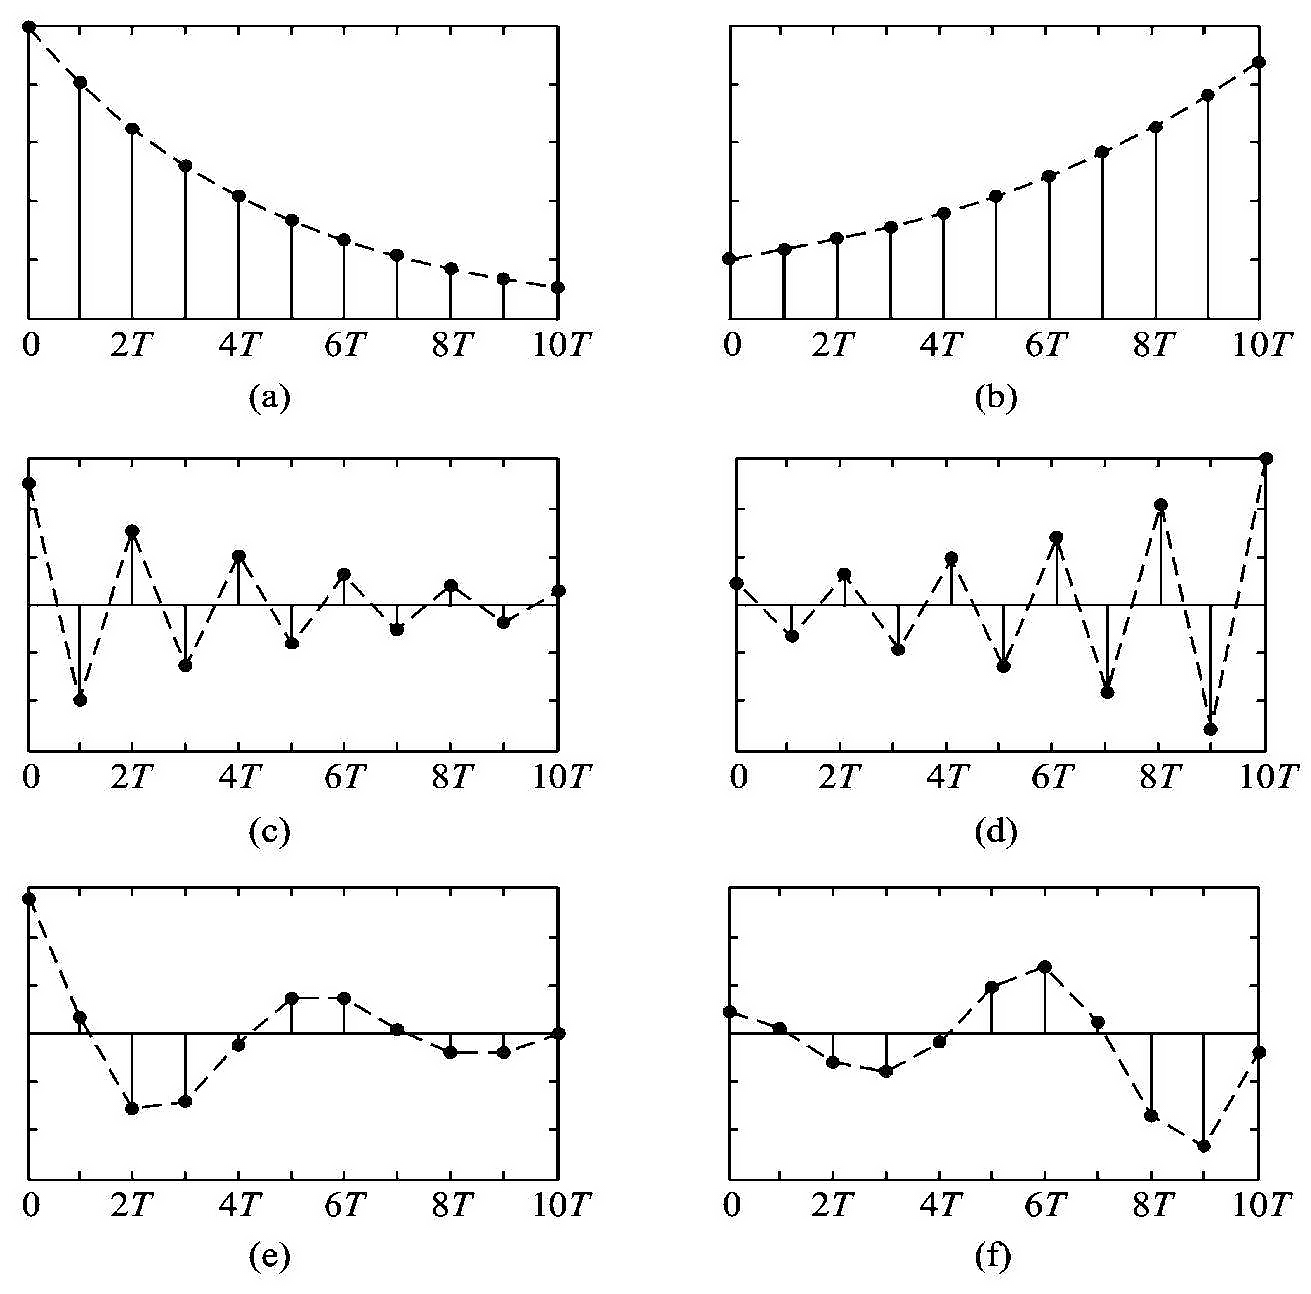
\includegraphics[width=0.58\linewidth]{pic/极点与瞬态响应.jpg}
	\vspace*{-1.5em}
	\caption{不同极点所对应的瞬态响应}
	\label{极点与瞬态响应}
\end{figure}

\noindent 如图\ref{极点与瞬态响应},下面分五种情况进行讨论
\begin{enumerate}[\hspace*{2em}(a) ]
	\item $0<p_k<1$\quad 极点所对应的瞬态分量是单调收敛的
	\item $p_k>1$\quad 极点所对应的瞬态分量是单调发散的
	\item $-1<p_k<0$ \quad 极点所对应的瞬态分量是正负交替的
	\item $p_k<-1$\quad 极点所对应的瞬态分量是正负交替的
	\item $p_k, p_{k+1}$为一对共轭复根,且$|p_k|<1$\quad 极点所对应的瞬态分量是按余弦规律振荡
	\item $p_k, p_{k+1}$为一对共轭复根,且$|p_k|>1$\quad 极点所对应的瞬态分量是按余弦规律振荡
\end{enumerate}
\vspace*{1em}

\subsection{稳态误差}

\begin{figure}[!htb]
	\centering
	\begin{tikzpicture}[circuit ee IEC]
		\node[bulb] (O) [draw, inner sep = 5pt, label = -85:$-$]{};
		\node (A) [draw, inner sep =6pt, right of = O, node distance =3cm]{$G(s)$};
		\node (B) [draw, inner sep = 6pt, below of = A, node distance = 1.5cm]{$H(s)$};
		
		\draw[arrows = {-Stealth}] (-1cm,0cm) -- (O)node[near start, above = 0mm]{$r(t)$};
		\draw (O) -- (1cm, 0cm) node[midway, above = 0mm]{$e(t)$} -- (1.5cm, 0.2cm);
		\draw[arrows = {-Stealth}] (1.5cm,0cm) -- (A)node[midway, above = 0cm]{$e^*(t)$};
		\draw[arrows = {-Stealth}] (A) --+(3cm, 0cm) node[very near end, xshift = 0.6cm]{$c(t)$};;
		\draw[arrows = {-Stealth}] (4.3cm, 0cm) -- +(0cm, -1.5cm) -- (B);
		\draw[arrows = {-Stealth}] (B) -- (0cm, -1.5cm) -- (O);
		\draw[dashed] (4.3cm,0cm) -- (4.3cm, 0.7cm)  -- (4.8cm, 0.7cm);
		\draw (4.8cm, 0.7cm) -- (5.3cm, 0.9cm);
		\draw[arrows = {-Stealth}, dashed] (5.3cm, 0.7cm) -- (6cm, 0.7cm)node[very near end, xshift = 0.5cm]{$c^*(t)$};
		
	\end{tikzpicture}
	\caption{闭环系统的稳态误差}
	\label{闭环稳态误差}
\end{figure}
如图\ref{闭环稳态误差},在输入信号$r(t)$作用下,误差的$z$变换的表达式为
\begin{equation}
	E(z) = \dfrac{1}{1+G(z)}R(z)
\end{equation}

\noindent \textbf{1. 当输入为阶跃函数时}
\begin{equation}
	R(z) = \dfrac{z}{z-1}
\end{equation}

定义\dy[静态位置误差系数]{JTWZWCXS}为
\begin{equation}
	K_p = \lim\limits_{z \to 1} G(z)
\end{equation}
则根据终值定理,有
\begin{equation}
	e(\infty) = \lim\limits_{z \to 1} (z - 1)\dfrac{1}{1 + G(z)} \cdot \dfrac{z}{z-1} = \dfrac{1}{1+K_p}
\end{equation}
\vspace*{0.5em}

\noindent \textbf{2. 当输入为单位斜坡函数时}
\begin{equation}
	R(z) = \dfrac{Tz}{(z-1)^2}
\end{equation}

定义\dy[静态速度误差系数]{JTSDWCXS}为
\begin{equation}
	K_v = \lim\limits_{z \to 1} (z-1)G(z)
\end{equation}
则根据终值定理,有
\begin{equation}
	e(\infty) = \lim\limits_{z \to 1} (z - 1)\dfrac{1}{1 + G(z)} \cdot \dfrac{Tz}{(z-1)^2} = \dfrac{T}{K_v}
\end{equation}
\vspace*{0.5em}

\noindent \textbf{3. 当输入为单位加速度信号时}
\begin{equation}
	R(z) = \dfrac{T^2z(z+1)}{2(z-1)^3}
\end{equation}

定义\dy[静态加速度误差系数]{JTJSDWCXS}为
\begin{equation}
	K_a = \lim\limits_{z \to 1} (z-1)^2G(z)
\end{equation}
则根据终值定理,有
\begin{equation}
	e(\infty) = \lim\limits_{z \to 1} (z - 1)\dfrac{1}{1 + G(z)} \cdot \dfrac{T^z(z+1)}{2(z-1)^3} = \dfrac{T^2}{K_a}
\end{equation}

总结如下表\ref{三个误差与输入信号的关系}.
\begin{table}[!htb]
	\centering
	\setlength{\tabcolsep}{8mm}{
		\begin{tabular}{ccccc}
			\toprule
			& & & & \vspace*{-1.3em} \\ 
			系统型别 & 静态误差系数 & $r(t) = 1(t)$ & $r(t) = t$ & $r(t) = \dfrac{1}{2}t^2$ \\
			& & & & \vspace*{-1.3em} \\
			\midrule
			& & & & \vspace*{-1.3em} \\
			0型系统 & 
			$\begin{aligned}
				K_\text{p} &= K\\
				K_\text{v} &= 0\\
				K_\text{a} &= 0
			\end{aligned}$
			& $e_{\text{ss}} = \dfrac{1}{1+K}$
			& $e_{\text{ss}} = \infty$
			& $e_{\text{ss}} = \infty$\\
			& & & & \vspace*{-1.2em} \\
			\hline
			& & & & \vspace*{-1.2em} \\
			\RMN[1] 型系统 &
			$\begin{aligned}
				K_\text{p} &= \infty\\
				K_\text{v} &= K\\
				K_\text{a} &= 0
			\end{aligned}$
			& $e_{\text{ss}} = 0$
			& $e_{\text{ss}} = \dfrac{T}{K}$
			& $e_{\text{ss}} = \infty$\\
			& & & & \vspace*{-1.2em} \\
			\hline
			& & & & \vspace*{-1.2em} \\
			\RMN[2] 型系统 &
			$\begin{aligned}
				K_\text{p} &= \infty\\
				K_\text{v} &= \infty \\
				K_\text{a} &= K
			\end{aligned}$
			& $e_{\text{ss}} = 0$
			& $e_{\text{ss}} = 0$
			& $e_{\text{ss}} = \dfrac{T^2}{K}$\\
			& & & & \vspace*{-1.2em} \\
			\hline
			& & & & \vspace*{-1.2em} \\
			\RMN[3] 型系统 &
			$\begin{aligned}
				K_\text{p} &= \infty\\
				K_\text{v} &= \infty\\
				K_\text{a} &= \infty
			\end{aligned}$
			& $e_{\text{ss}} = 0$
			& $e_{\text{ss}} = 0$
			& $e_{\text{ss}} = 0$\\
			& & & & \vspace*{-1.2em} \\
			\bottomrule
		\end{tabular}
	}
	\caption{稳态误差、静态误差系数与输入信号之间的关系}
	\label{三个误差与输入信号的关系}
\end{table}

\examples \label{7.11}已知采样系统的结构如图所示,其中
$$
G(s) = \dfrac{2(0.5s + 1)}{s^2}
$$
采样周期$T=0.2\,\text{s}$,求在输入信号$r(t) = 1+t+0.5t^2(t>0)$的作用下,系统的稳态误差。
	\begin{figure}[!htb]
	\centering
	\begin{tikzpicture}[circuit ee IEC]
		\node (A)[draw, inner sep = 6pt, xshift = 1.6cm]{ZOH};
		\node (B) [draw, inner sep =5pt, right of = A, node distance = 2.4cm]{$G_2(s)$};
		\node[bulb] (O)[draw, inner sep = 6pt, xshift = -1.8cm, label = -85:$-$]{};
		
		\draw[arrows={-Stealth}] (-3cm,0cm) -- (O)node[near start, above = 0cm]{$r(t)$};
		\draw[arrows={-Stealth}] (0cm,0cm) --(A);
		\draw[arrows={-Stealth}] (A) -- (B);
		\draw[arrows={-Stealth}] (B) --+(3cm,0cm)node[midway, above = 0cm]{$c(t)$};
		\draw (-1.5cm, 0cm) -- (-0.5cm,0cm);
		\draw (-0.5cm, 0cm) -- (0cm,0.2cm);		
		\draw (6cm,0cm) -- +(0cm,-1cm) -- (-1.8cm,-1cm) -- (O);
		
	\end{tikzpicture}
	\caption{\ref{7.11}$\,$ 系统结构图}
	\label{7.11-1}
\end{figure}

\solve 采样系统的开环传递函数为
\begin{align*}
	G(z) &= \left(1 - z^{-1}\right)\cdot Z\Bigg[\dfrac{1}{s}\cdot \dfrac{2(0.5s+1)}{s^2}\Bigg]\\[0.5em]
	& = \dfrac{z-1}{z}\Bigg[\dfrac{Tz}{(z-1)^2}+ \dfrac{T^2z(z+1)}{(z-1)^3}\Bigg]\\[0.5em]
	& = \dfrac{0.24z - 0.16}{(z-1)^2}
\end{align*}

\textbf{(求稳态误差前一定要判断系统的稳定性)}采样系统的闭环特征方程为
\[
D(z) = z^2 - 1.76z + 0.84 = 0
\]
所以,$D(1) = 0.08>0,\quad D(-1) = 3.6>0\quad |a_0|=0.84<a_2=1$,即系统稳定。

由于系统的传递函数存在两个$(z-1)^{-1}$,即此为\RMN[2]型系统,则
\begin{align*}
	K_\text{p} &= 0\\
	K_\text{v} &= 0\\
	K_\text{a} & = \lim\limits_{z \to 1}(z-1)^2G(z) = \lim\limits_{z \to 1}(0.24z-0.16) = 0.08
\end{align*}
所以,在输入$r(t)=1+t+0.5t^2$作用下的稳态误差为
\[
e(\infty) = \dfrac{1}{1+K_\text{p}} + \dfrac{T}{K_\text{v}}+\dfrac{T^2}{K_\text{a}} = 0 + 0 + \dfrac{0.04}{0.08} = 0.5
\]

\section{采样系统的数字校正}
\begin{figure}[!htb]
	\centering
	\begin{tikzpicture}[circuit ee IEC]
		\node[bulb] (O) [draw, inner sep =6pt, label = -85:$-$]{};
		\node (A) [draw, right of = O, inner sep = 5pt, node distance = 3cm]{$D(z)$};
		\node (B) [draw, right of = A, inner sep = 5pt, node distance = 3cm]{$G(s)$};
		
		\draw[arrows={-Stealth}] (-1.2cm,0cm) -- (O)node[near start, above = 0cm]{$r(t)$};
		\draw (O) -- (1cm,0cm)node[midway, above = 0cm]{$e(t)$} -- (1.5cm,0.2cm);
		\draw [arrows={-Stealth}] (1.5cm, 0cm) -- (A)node[midway, above = 0cm]{$e^*(t)$};
		\draw (A) -- +(1.2cm,0cm)node[midway, above = 0cm, xshift = 1mm]{$u(t)$} -- +(1.7cm,0.2cm);
		\draw [arrows={-Stealth}] (4.7cm, 0cm) -- (B)node[midway, above = 0cm]{$u^*(t)$};
		\draw [arrows={-Stealth}](B) --+ (2.5cm, 0cm)node[midway, above = 0cm]{$c(t)$};
		\draw [arrows={-Stealth}](7.5cm,0cm) --+(0cm, -1cm) -- (0cm ,-1cm) -- (O);
		
	\end{tikzpicture}
\caption{含数字校正装置的采样系统}
\label{数字校正}
\end{figure}

如图\ref{数字校正}所示的闭环采样系统,闭环脉冲传递函数为
\begin{equation}
	\varPhi(z) = \dfrac{G(z)D(z)}{1+G(z)D(z)}
\end{equation}
系统的误差为
\begin{equation}
	E(z) = R(z) - C(z) = \left[1 - \varPhi(z)\right]R(z)
\end{equation}

设输入为时间的幂函数$At^q(t>0)$,其中$q$是正整数,则
\begin{equation}
	R(z) = \dfrac{B(z)}{\big(1-z^{-1}\big)^{q+1}}
\end{equation}
其中,$B(z)$是$z^{-1}$的有限次多项式.
\vspace*{0.5em}

为了使稳态误差
\begin{equation}
	e(\infty) = \lim\limits_{z\to 1}\big(1-z^{-1}\big)E(z) = \lim\limits_{z\to 1}\big(1-z^{-1}\big)\left[1-\varPhi(z)\right]R(z) = \lim\limits_{z\to 1}\left[1-\varPhi(z)\right]\dfrac{B(z)}{\big(1-z^{-1}\big)^{q}} = 0
\end{equation}
则$1-\varPhi(z)$项至少有$q+1$个$(1-z^{-1})$因子,不妨取$q+1$个,即可以写为
\begin{equation}
	1-\varPhi(z) = \big(1-z^{-1}\big)^{q+1}\varphi(z)
\end{equation}
其中,$\varphi(z)$是关于$z^{-1}$的多项式,并且不含因子$\big(1-z^{-1}\big)$.
\vspace*{0.5em}

又为了使系统能在尽可能少的周期内实现对输入的完全跟踪,应使中$\varphi(z)$所含$z^{-1}$项的数目最少,为此应取$\varphi(z) = 1$,即
\begin{equation}
	\varPhi(z) = 1 - \big(1-z^{-1}\big)^{q+1}\varphi(z) \xlongequal{\textstyle \quad \varphi(z) = 1\quad}  1 - \big(1-z^{-1}\big)^{q+1}
\end{equation}
代入脉冲传递函数,可得
\begin{equation}
	D(z) = \dfrac{1}{G(z)}\dfrac{\varPhi(z)}{1 - \varPhi(z)}
\end{equation}

特别地,此时误差函数的$z$变换为
\begin{equation}
	E(z) = R(z) - C(z) = \left[1 - \varPhi(z)\right]R(z) = \big(1-z^{-1}\big)^{q+1}\varphi(z) \cdot \dfrac{B(z)}{\big(1-z^{-1}\big)^{q+1}} = \varphi(z)B(z)\xlongequal{\textstyle \quad \varphi(z) = 1\quad} B(z)
\end{equation}

\noindent 下面以输入为阶跃、斜坡和等加速度函数时的情形。
\begin{enumerate}[\hspace*{2em} 1. ]
	\item $\bm{r(t) = 1(t)}$
	\begin{equation}
		R(z) = \dfrac{z}{z-1} = \dfrac{1}{\big(1-z^{-1}\big)^{0+1}} = \dfrac{B(z)}{\big(1-z^{-1}\big)^{q+1}}
	\end{equation}
	最少拍无差系统的闭环传递函数为
	\begin{equation}
		\varPhi(z) = 1 - \big(1-z^{-1}\big)^{0+1} = z^{-1}
	\end{equation}
	此时误差信号的$z$变换为
	\begin{equation}
		E(z) = B(z) = 1 = 1\cdot z^0
	\end{equation}
	系统经过\textcolor{blue}{1拍}便可以完全跟踪上输入信号。
	\vspace*{0.5em}
	
	\item $\bm{r(t) = t}$
	\begin{equation}
		R(z) = \dfrac{Tz}{(z-1)^2} = \dfrac{Tz^{-1}}{\big(1-z^{-1}\big)^{1+1}} = \dfrac{B(z)}{\big(1-z^{-1}\big)^{q+1}}
	\end{equation}
	最少拍无差系统的闭环传递函数为
	\begin{equation}
		\varPhi(z) = 1 - \big(1-z^{-1}\big)^{1+1} = 2z^{-1} - z^{-2}
	\end{equation}
	此时误差信号的$z$变换为
	\begin{equation}
		E(z) = B(z) = T z^{-1}
	\end{equation}
	系统经过\textcolor{blue}{2拍}便可以完全跟踪上输入信号。
	\vspace*{1em}
	
	\item $\bm{r(t) = \dfrac{1}{2}t^2}$
	\begin{equation}
		R(z) = \dfrac{T^2z(z+1)}{2(z-1)^3} = \dfrac{0.5T^2(z^{-1}+z^{-2})}{\big(1-z^{-1}\big)^{2+1}} = \dfrac{B(z)}{\big(1-z^{-1}\big)^{q+1}}
	\end{equation}
	最少拍无差系统的闭环传递函数为
	\begin{equation}
		\varPhi(z) = 1 - \big(1-z^{-1}\big)^{2+1} = 3z^{-1} - 2z^{-2} + z^{-3}
	\end{equation}
	此时误差信号的$z$变换为
	\begin{equation}
		E(z) = B(z) = 0.5T^2(z^{-1}+z^{-2})
	\end{equation}
	系统经过\textcolor{blue}{3拍}便可以完全跟踪上输入信号。
\end{enumerate}

























